\section{Jet Response}
\subsection{Introduction}
\label{sec:jetresponse}
In this section we look at performance plots for jet reconstruction using ITS-only tracking. Since the momentum resolution of ITS-only is worse than that of TPC+ITS (see Figure ~\ref{fig:resolution}), it will have an impact in the momentum resolution of the jets reconstructed from using ITS-only tracks. As mentioned in Section~\ref{sec:jetreco}, our ``truth" jets are composed of only charged-particles.  

In order to obtain the jet \pt~resolution, we use the pp and p-Pb $\gamma$-jet  and  Monte Carlo (LHC17g6a1 and LHC18g10a) mentioned in table~\ref{tab:MCsamples} to obtain the true jet transverse momentum (\pt$^{\mathrm{true}}$) and the recconstructed jet momentum (\pt$^{\mathrm{reco}}$). For the purpose of this study, we only select jets with {$|\eta| < 0.5$} and with {$\pt^{\mathrm{reco}} > 5$ \GeVc} in order to be consistent with the cuts applied on the jets for the isolated photon-jet correlations (section~\ref{sec:GammaJet}).

%In order to study the effects of the ITS holes on the jet angular distribution and efficiencies, we used the pp and p-Pb $\gamma$-jet Monte Carlo (LHC17g6a1 and LHC18b10a) mentioned in table~\ref{tab:MCsamples}.

\subsection{True and Reco jet $\pt$ comparison}
The jet momentum resolution is the spread in the variable, $100 (p_\mathrm{T,ch \: jet}^{reco} - p_\mathrm{T,ch \: jet}^{truth})/p_\mathrm{T,ch \: jet}^{truth}$, as a function of $p_\mathrm{T,ch \: jet}^{truth}$. Figure~\ref{fig:jetResolution} shows the momentum resolution of charged jet \pt.The means of the distributions in Figure~\ref{fig:jetResolution} are found in Table~\ref{tab:ptresolStat} which indicates that tracking inefficiencies reduce our ability to reconstruct charged tracks. Since we miss tracks due to the tracking inefficiency, those tracks cannot contribute to the jet $p_\mathrm{T,ch \: jet}^{reco}$, thus $p_\mathrm{T,ch \: jet}^{reco}$ is less than $p_\mathrm{T,ch \: jet}^{truth}$.
\begin{figure}[h]
\center
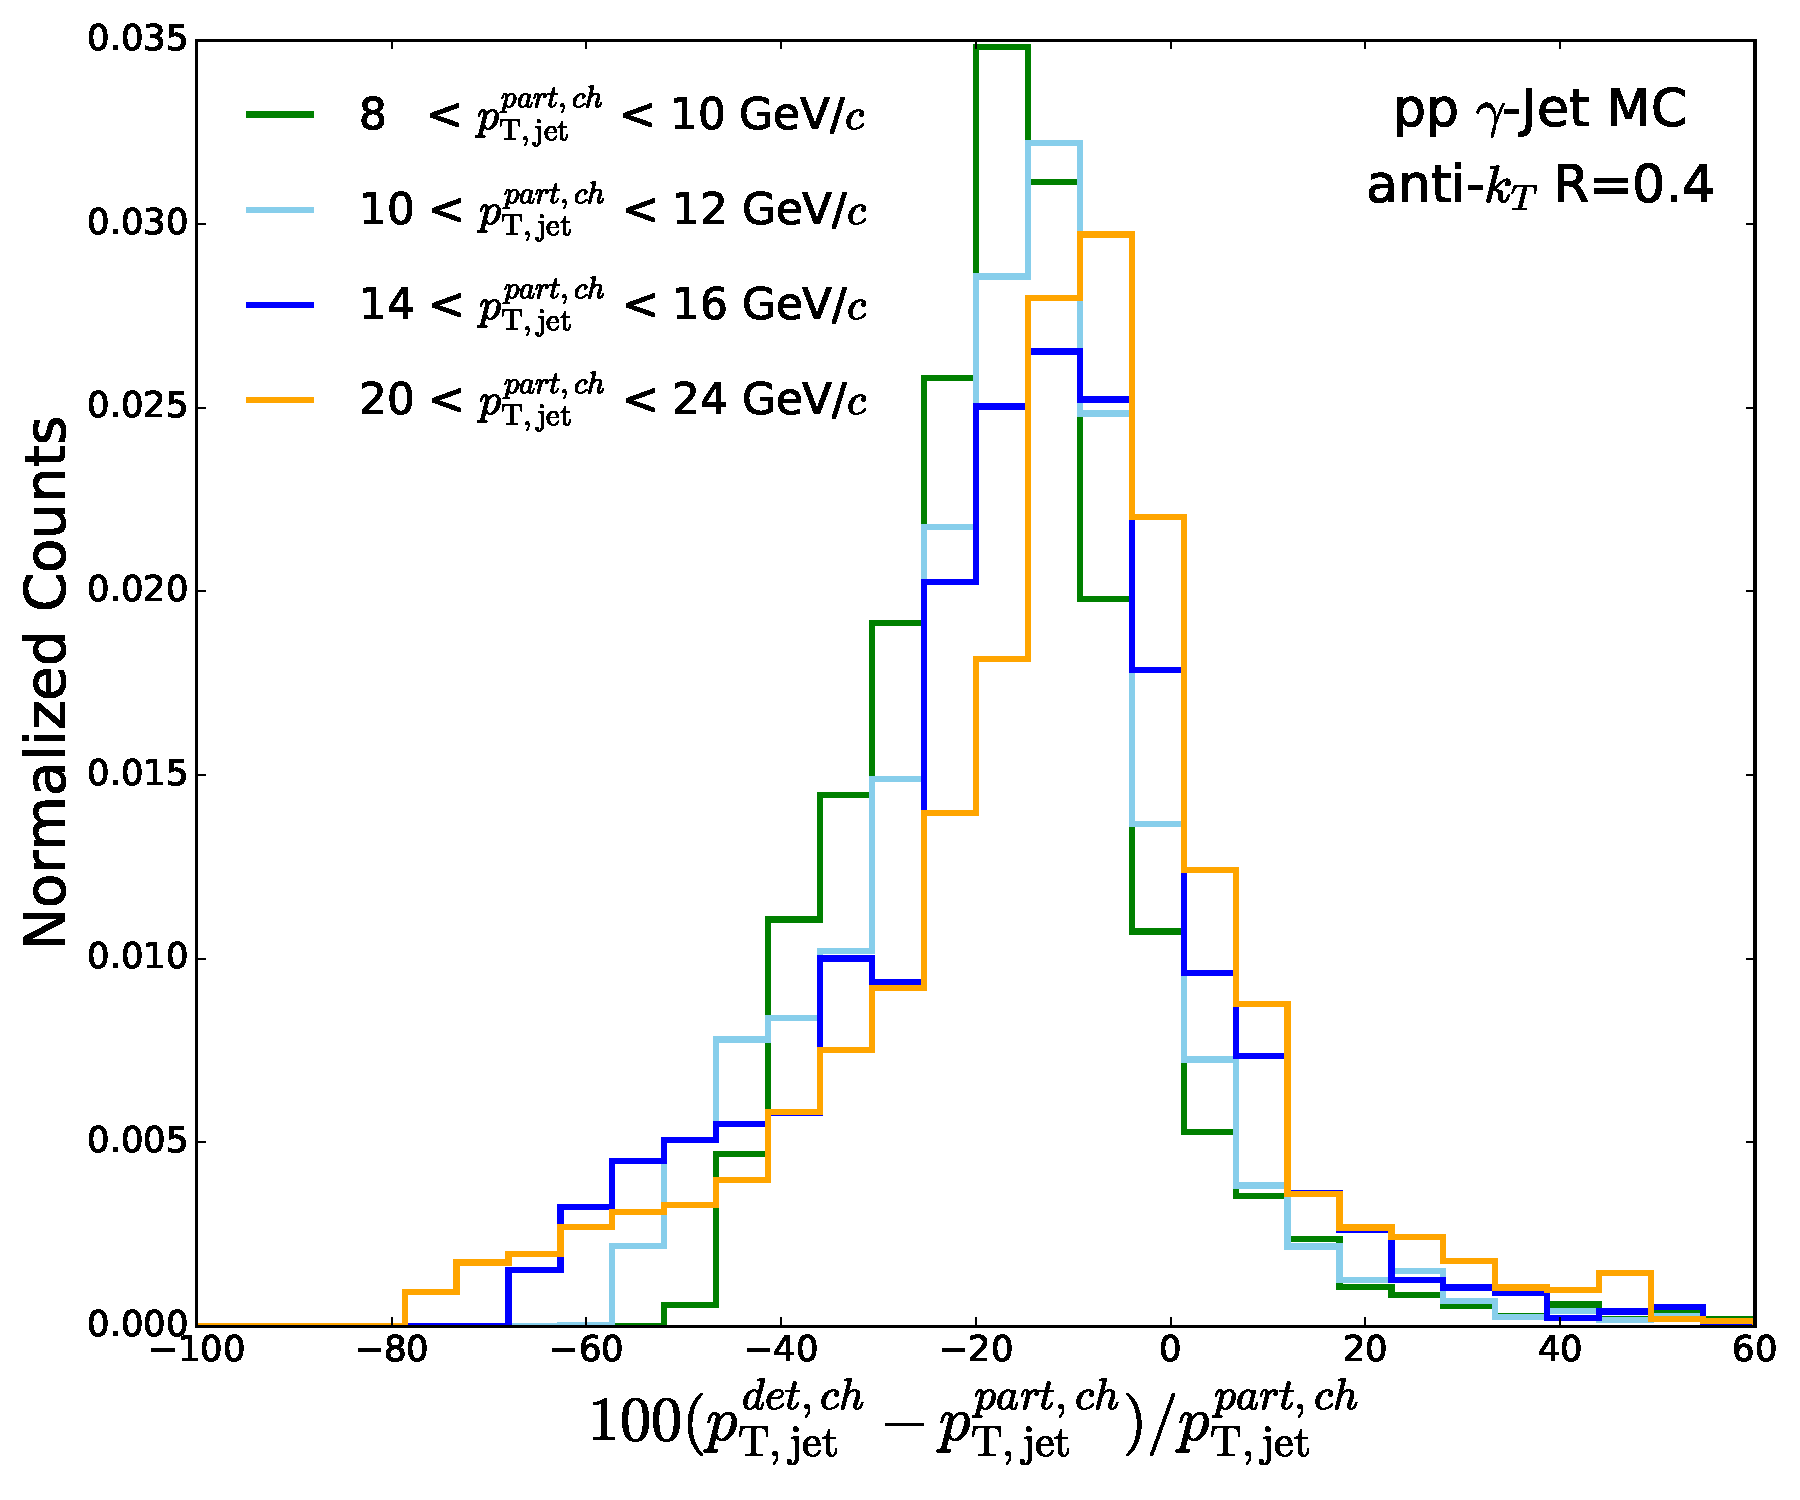
\includegraphics[width=0.55\textwidth]{JetResponse/pp_MC_pt_resol.pdf}
\caption{The resolution of the jet momentum for the various $p_\mathrm{T,ch \: jet}^{truth}$ slices for ITS-only charged jet in pp $\gamma$-Jet MC simulation (LHC18b10a).}
\label{fig:jetResolution}
\end{figure}
\begin{table}[h]
   \centering
   \caption{The root mean square and mean of the jet transverse momentum resolution distributions of different $p_\mathrm{T,ch \: jet}^{truth}$ ranges in pp $\gamma$-Jet MC simulation (LHC18b10a).}
    \label{tab:ptresolStat}
    \begin{tabular*}{0.9\columnwidth}{@{\extracolsep{\fill}}lcc@{}}
    \hline
    & RMS & Mean \\
    \hline
    $8 \:\:\: < p_\mathrm{T,ch \: jet}^{truth}  < 10$ \GeVc & 23\% & -16\% \\ 
    $10 < p_\mathrm{T,ch \: jet}^{truth} < 12$ \GeVc & 24\% & -17\% \\ 
    $14 < p_\mathrm{T,ch \: jet}^{truth}  < 16$ \GeVc & 24\% & -16\% \\ 
    $20 <p_\mathrm{T,ch \: jet}^{truth}  < 24$ \GeVc & 26\% & -14\% \\ 
	\hline
    \end{tabular*}
\end{table}

\begin{figure}[h]
    \center
	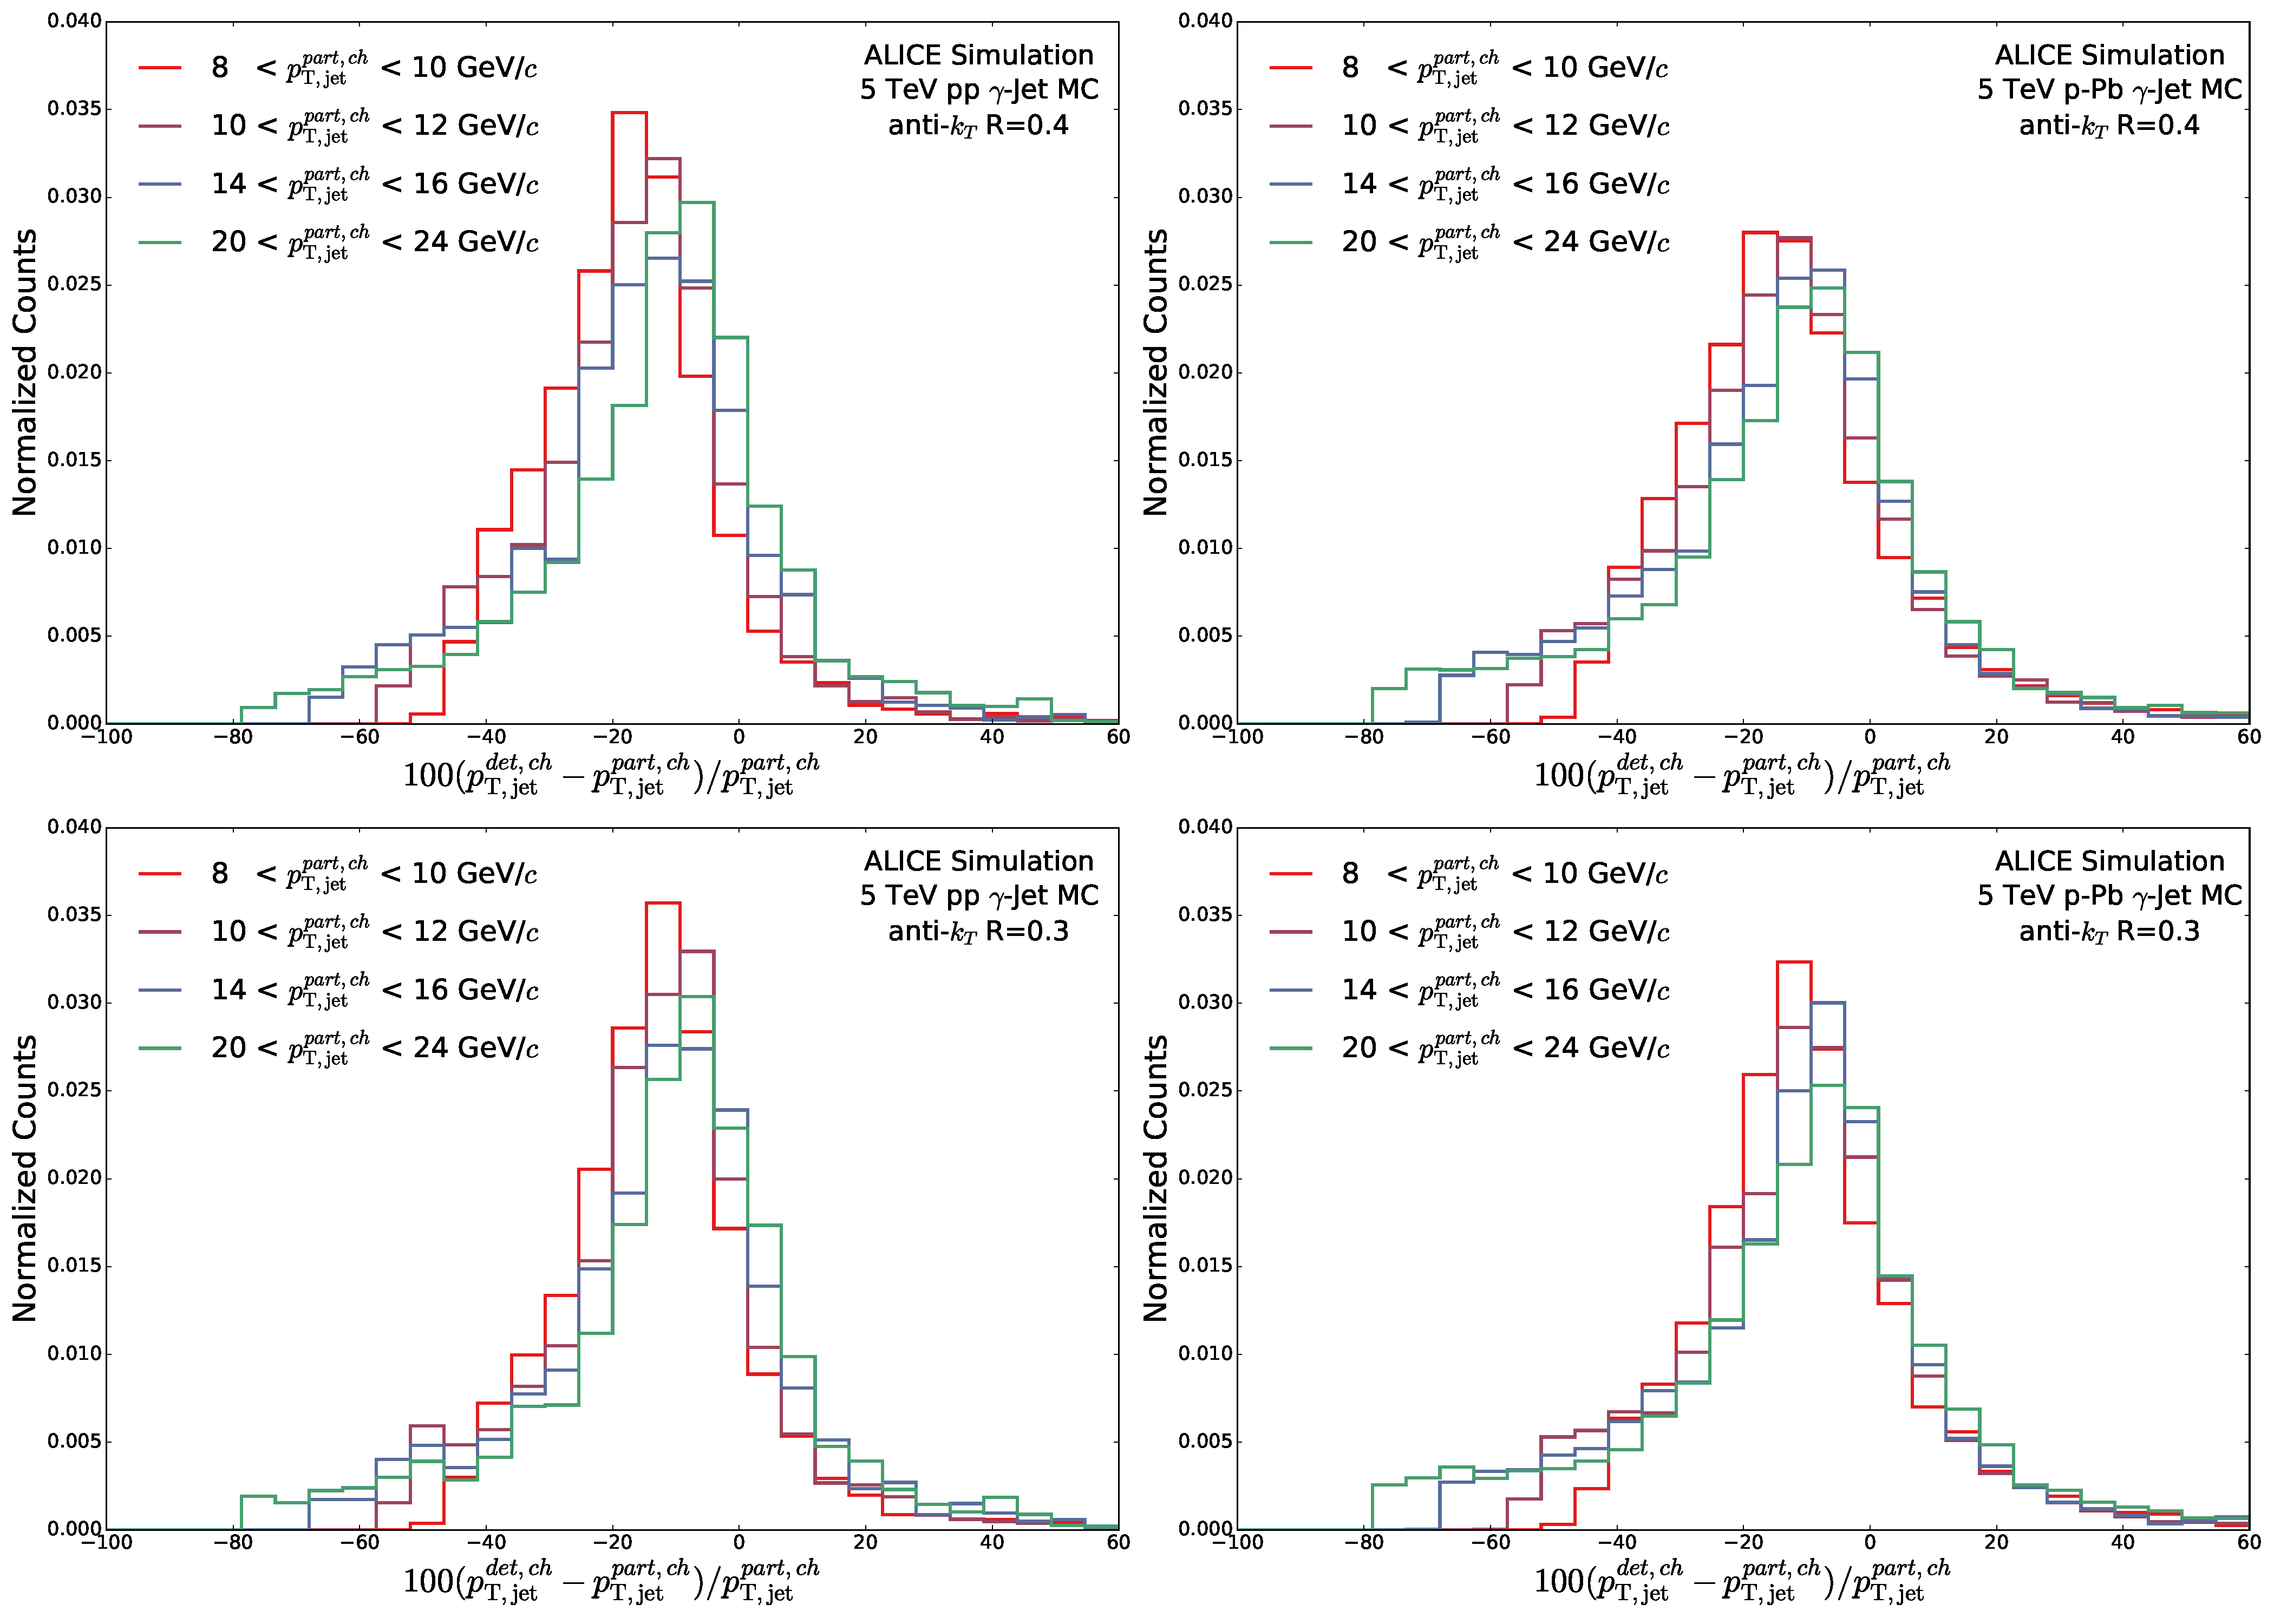
\includegraphics[width=1.0\textwidth]{JetResponse/jet_pt_resol_GJ.pdf}
	\caption{The jet transverse momentum resolution for different ranges in true jet transverse momentum of $\gamma$-Jet, using LHC17g6a1 and LHC18b10a for p-Pb and pp respectively, MC simulations for both reconstructed jets with R = 0.3 and R = 0.4.}
	\label{fig:jet_pt_resol_GJ}
\end{figure}
   
\begin{table}[h]
   \centering
   \caption{The standard deviation and mean of the jet transverse momentum resolution distributions of different $p_\mathrm{T,ch \: jet}^{truth}$ ranges using LHC17g6a1 and LHC18b10a for p-Pb and pp $\gamma$-jet MC simulations respectively.}
    \label{tab:ptresolStat}
    \begin{tabular*}{1.0\columnwidth}{@{\extracolsep{\fill}}lcccc@{}}
    \hline
    pp & $\sigma$ with R=0.4 & Mean with R=0.4 & $\sigma$ with R=0.3 & Mean with R=0.3 \\
    \hline
    $8 \:\:\: < p_\mathrm{T,ch \: jet}^{truth} < 10$ \GeVc & 15$\%$ & -16$\%$ & 15$\%$ & -12$\%$\\ 
    $10 < p_\mathrm{T,ch \: jet}^{truth} < 12$ \GeVc & 17$\%$ & -16$\%$ & 17$\%$ & -13$\%$\\ 
    $14 < p_\mathrm{T,ch \: jet}^{truth} < 16$ \GeVc & 19$\%$ & -15$\%$ & 20$\%$ & -12$\%$\\ 
    $20 < p_\mathrm{T,ch \: jet}^{truth} < 24$ \GeVc & 21$\%$ & -14$\%$ & 22$\%$ & -11$\%$\\ 
	\hline
	p-Pb & & & &  \\
    \hline
    $8 \:\:\: < p_\mathrm{T,ch \: jet}^{truth} < 10$ \GeVc & 18$\%$ & -13$\%$ & 17$\%$ & -10$\%$\\ 
    $10 < p_\mathrm{T,ch \: jet}^{truth} < 12$ \GeVc & 19$\%$ & -13$\%$  & 19$\%$ & -11$\%$\\ 
    $14 < p_\mathrm{T,ch \: jet}^{truth} < 16$ \GeVc & 21$\%$ & -14$\%$ & 22$\%$ & -12$\%$\\ 
    $20 < p_\mathrm{T,ch \: jet}^{truth} < 24$ \GeVc & 24$\%$ & -13$\%$ & 24$\%$ & -12$\%$\\ 
	\hline
    \end{tabular*}
\end{table}
\subsection{Jet \pt~Response matrix}
The response matrix for ITS jets in pp is shown in Figure~\ref{fig:jetResponseMatrix}. There is a visible linear correlation between \pt$^{\mathrm{true}}$ and \pt$^{\mathrm{reco}}$ starting at {\pt$^{\mathrm{true}} =$ 5 \GeVc}. The projections of both the axes of the response matrix are also shown in Figure~\ref{fig:jetResponseMatrix}. We can see from the projections that \pt$^{\mathrm{true}}$ is always greater than \pt$^{reco}$ past 8 GeV. While \pt$^{true}$ should always be greater than \pt$^{\mathrm{reco}}$, the dip at lower \pt~arises because we require \pt$^{reco} > 5$ \GeVc. This is because to detect a 5 GeV reco-jet, the \pt$^{\mathrm{true}}$ must be greater than 5~\GeVc. 
%bvj by a few GeV.
\begin{figure}[h]
\center
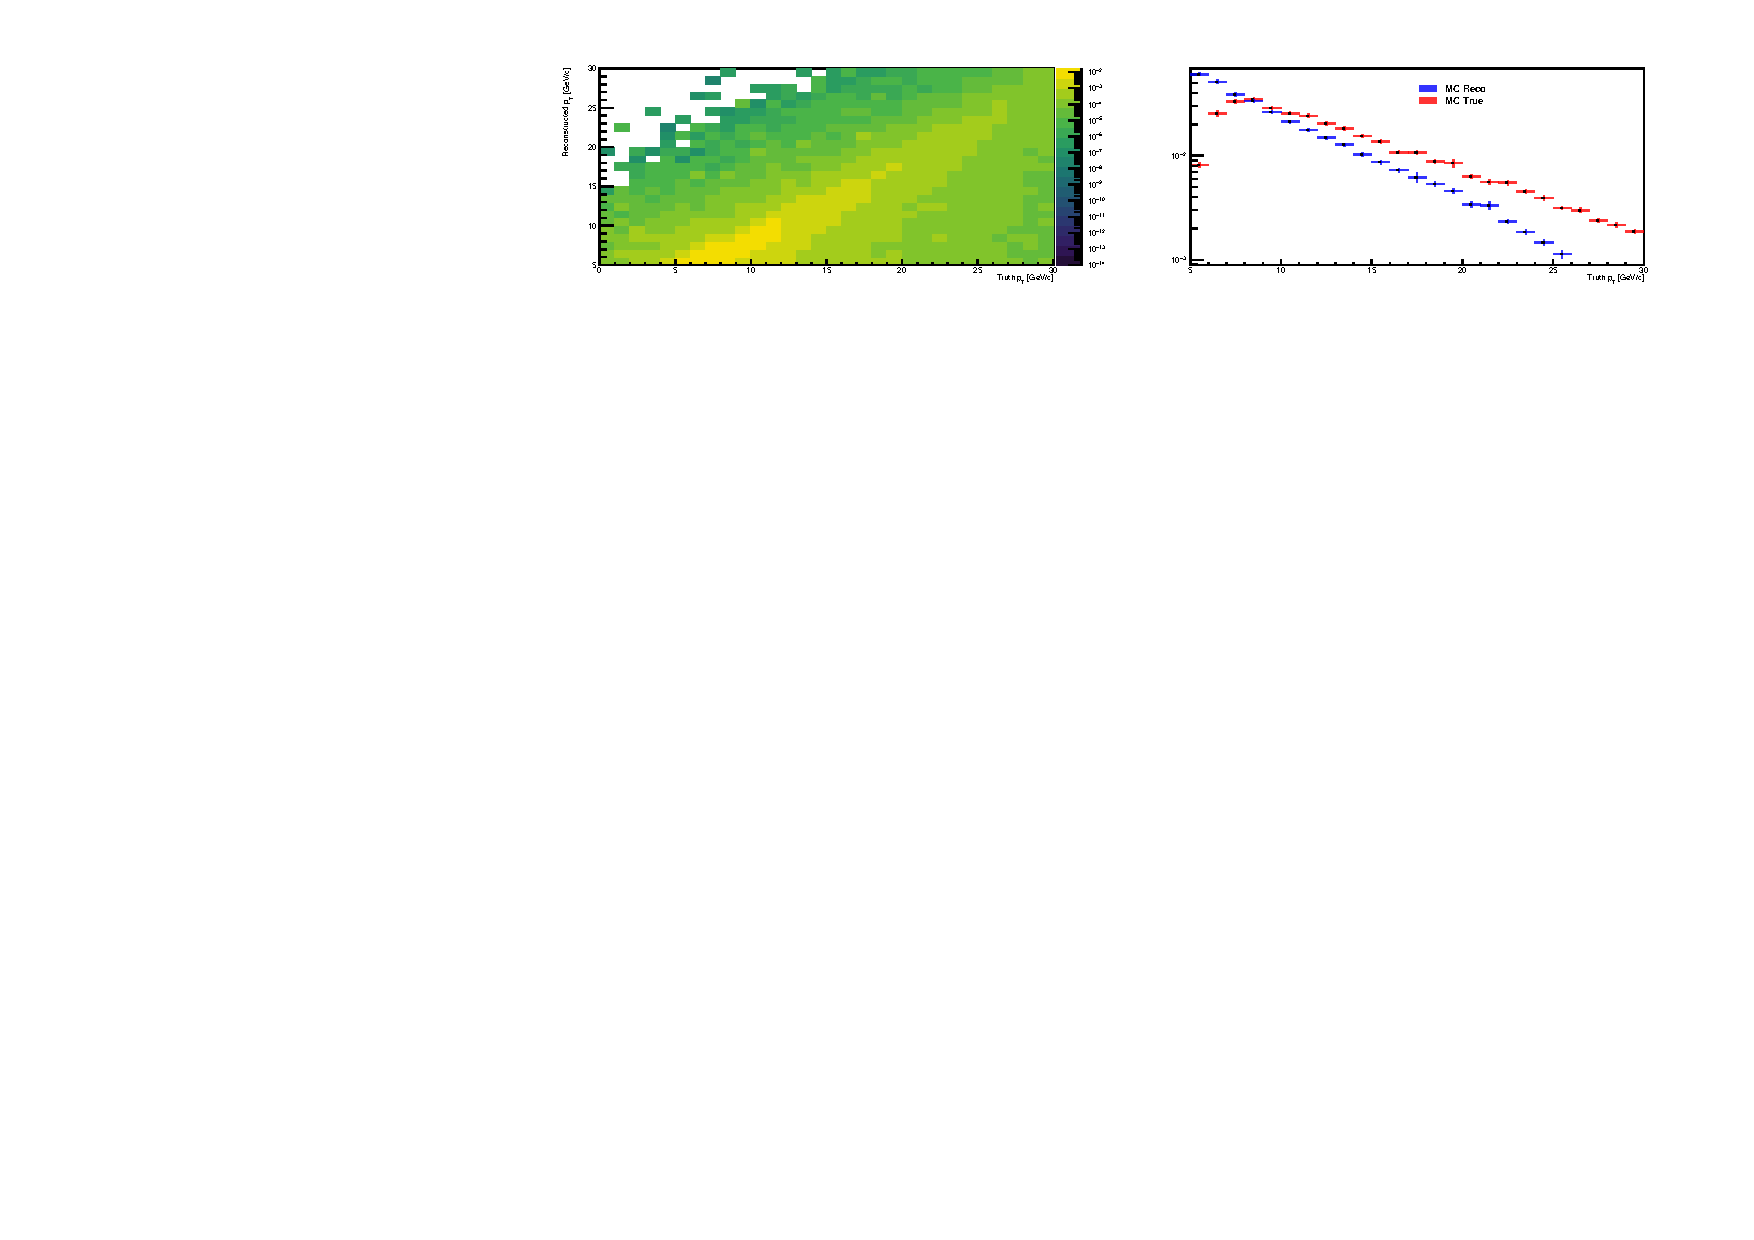
\includegraphics[height=0.5\textwidth,width=\textwidth]{JetResponse/Matrix_jets_its_pp.pdf}
\caption{The response matrix for \pt$^{\mathrm{jet}}$ which is a correlation matrix between \pt$^{\mathrm{true}}$ and \pt$^{\mathrm{reco}}$ (left), and the projections of the true and reco \pt~(right). The drop at low momentum for \pt$^{\mathrm{true}}$, labeled as MC True in the plot, is due the requirement $\pt^{\mathrm{reco}} > 5$ \GeVc. This response matrix is for pp, made using using LHC18g10a.} 
\label{fig:jetResponseMatrix}
\end{figure}
%bvj The matter 
That \pt$^{\mathrm{reco}}$ is always less than \pt$^{\mathrm{true}}$ is shown explictly in Figure~\ref{fig:jetResonseProjections}, which has projections of the response matrix for two different \pt$^{\mathrm{true}}$ slices onto the \pt$^{\mathrm{reco}}$ axis.
\begin{figure}[h]
\center
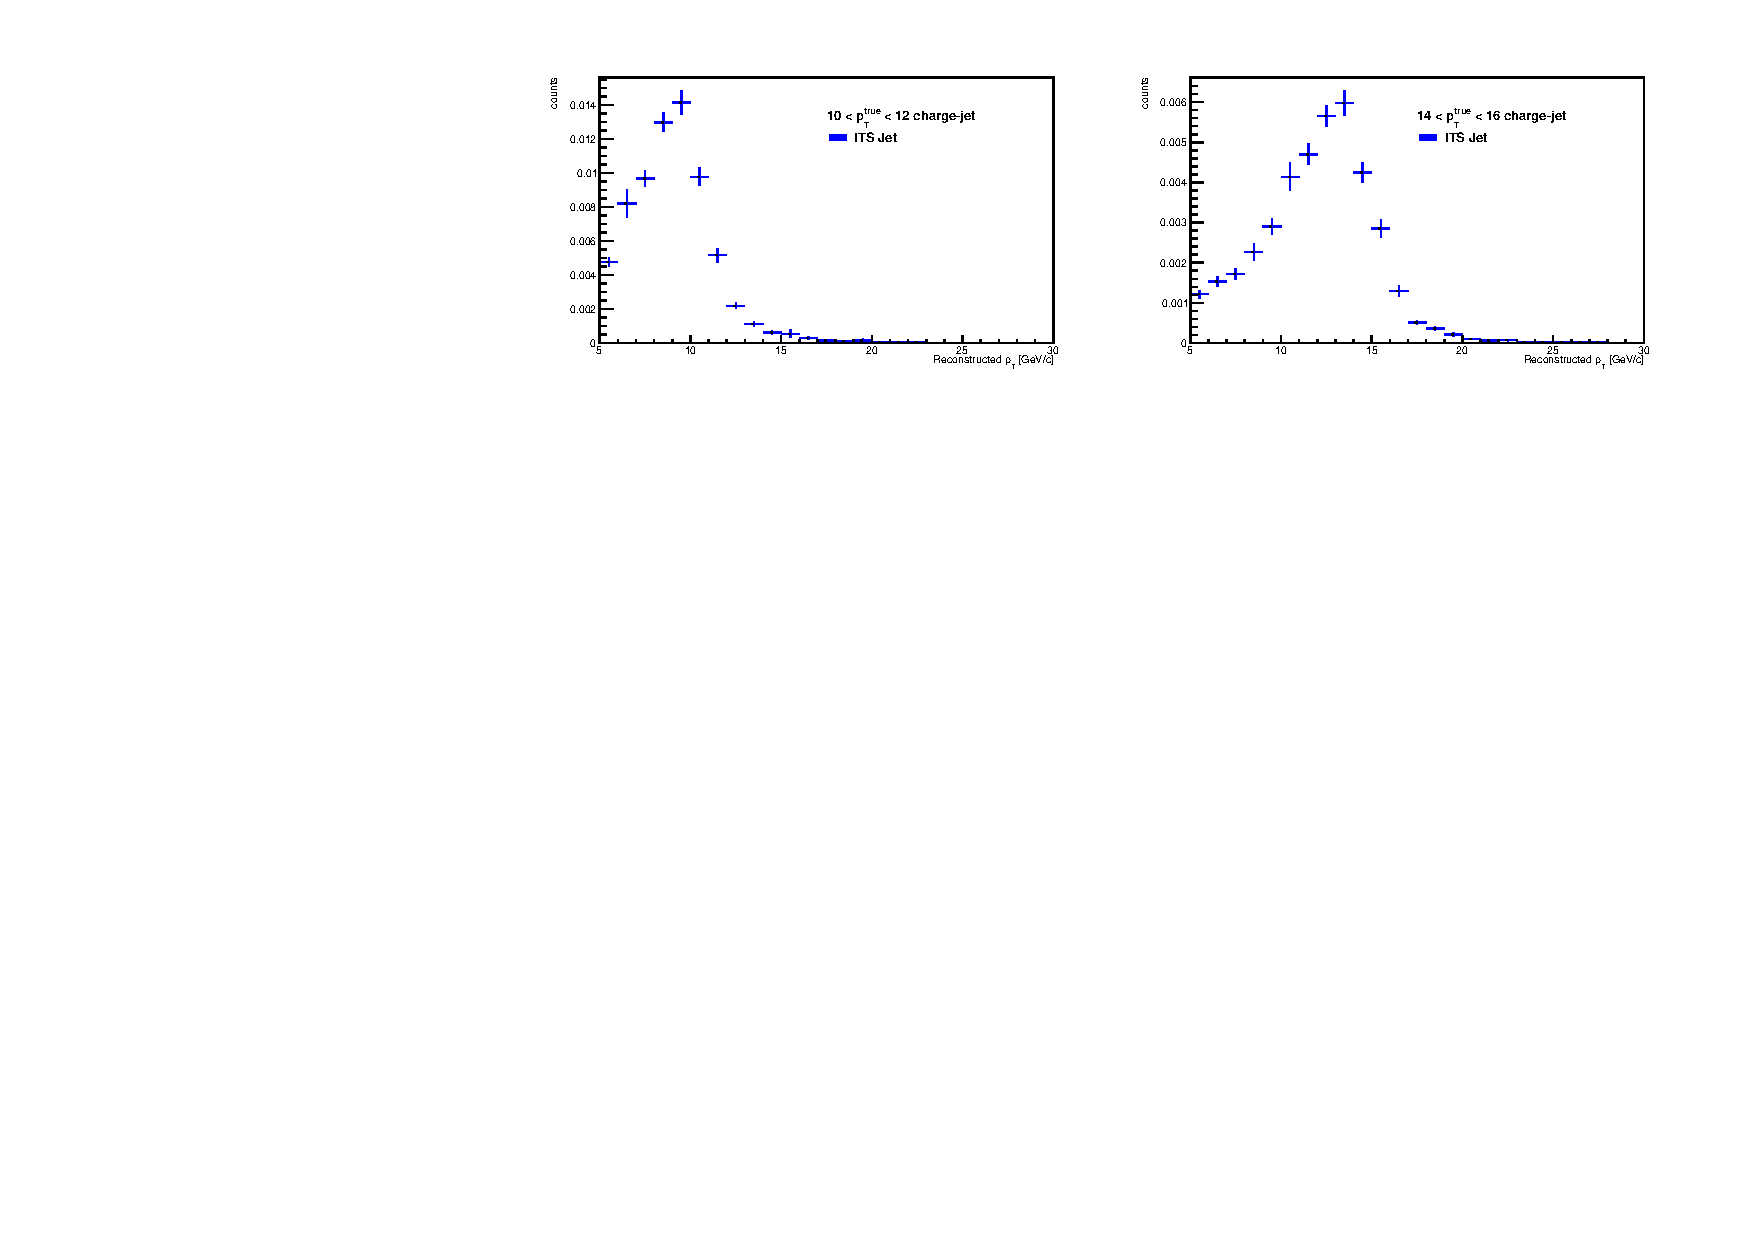
\includegraphics[height=0.45\textwidth, width=1.\textwidth]{JetResponse/fulljet_projections-10-14_pp.pdf}
\caption{Projections of $10 < \pt^{\mathrm{true}} < 12$ \GeVc bins (left) and $14 < \pt^{\mathrm{true}} < 16$ \GeVc bins on to \pt$^{\mathrm{reco}}$, using 18g10a for pp $\gamma$-jet MC. The peak of the projection is always lower than the \pt$^{\mathrm{true}}$ range as the 10--12 \GeVc \pt$^{\mathrm{true}}$ peaks at 9 GeV \pt$^{\mathrm{reco}}$, while the 14--16 \GeVc \pt$^{\mathrm{true}}$ peaks at 13--14 \GeVc \pt$^{\mathrm{true}}$.}  
\label{fig:jetResonseProjections}
\end{figure}

\subsection{Jet distribution in detector $\eta$ and $\phi$ acceptance}
As seen in Figure~\ref{fig:2Defficiency}, the ITS has holes in $\phi$ which caused us to lose tracks. Since jets are reconstructed from tracks, and we miss some of these, it is necessary to see the impact of the holes on the jet reconstruction. Additionally, the efficiency as a function of $\eta$ and $\phi$ as well as the smearing due ITS-only tracking on jets is also shown. 

Figure~\ref{fig:2Djets} shows the $\eta$ and $\phi$ values of the jets as obtained from the Monte Carlo. The jets are concentrated in the region $-$2 rad $< \phi <$ 0.5 rad because these are recoil jets opposite to a photon in the EMCal. We can see in the reconstructed $\eta$ and $\phi$ distributions, there are holes present in the p-Pb plots. The holes are not present in the pp plots because the staves in ITS were replaced, and so the holes were fixed. 

\begin{figure}[h]
\center
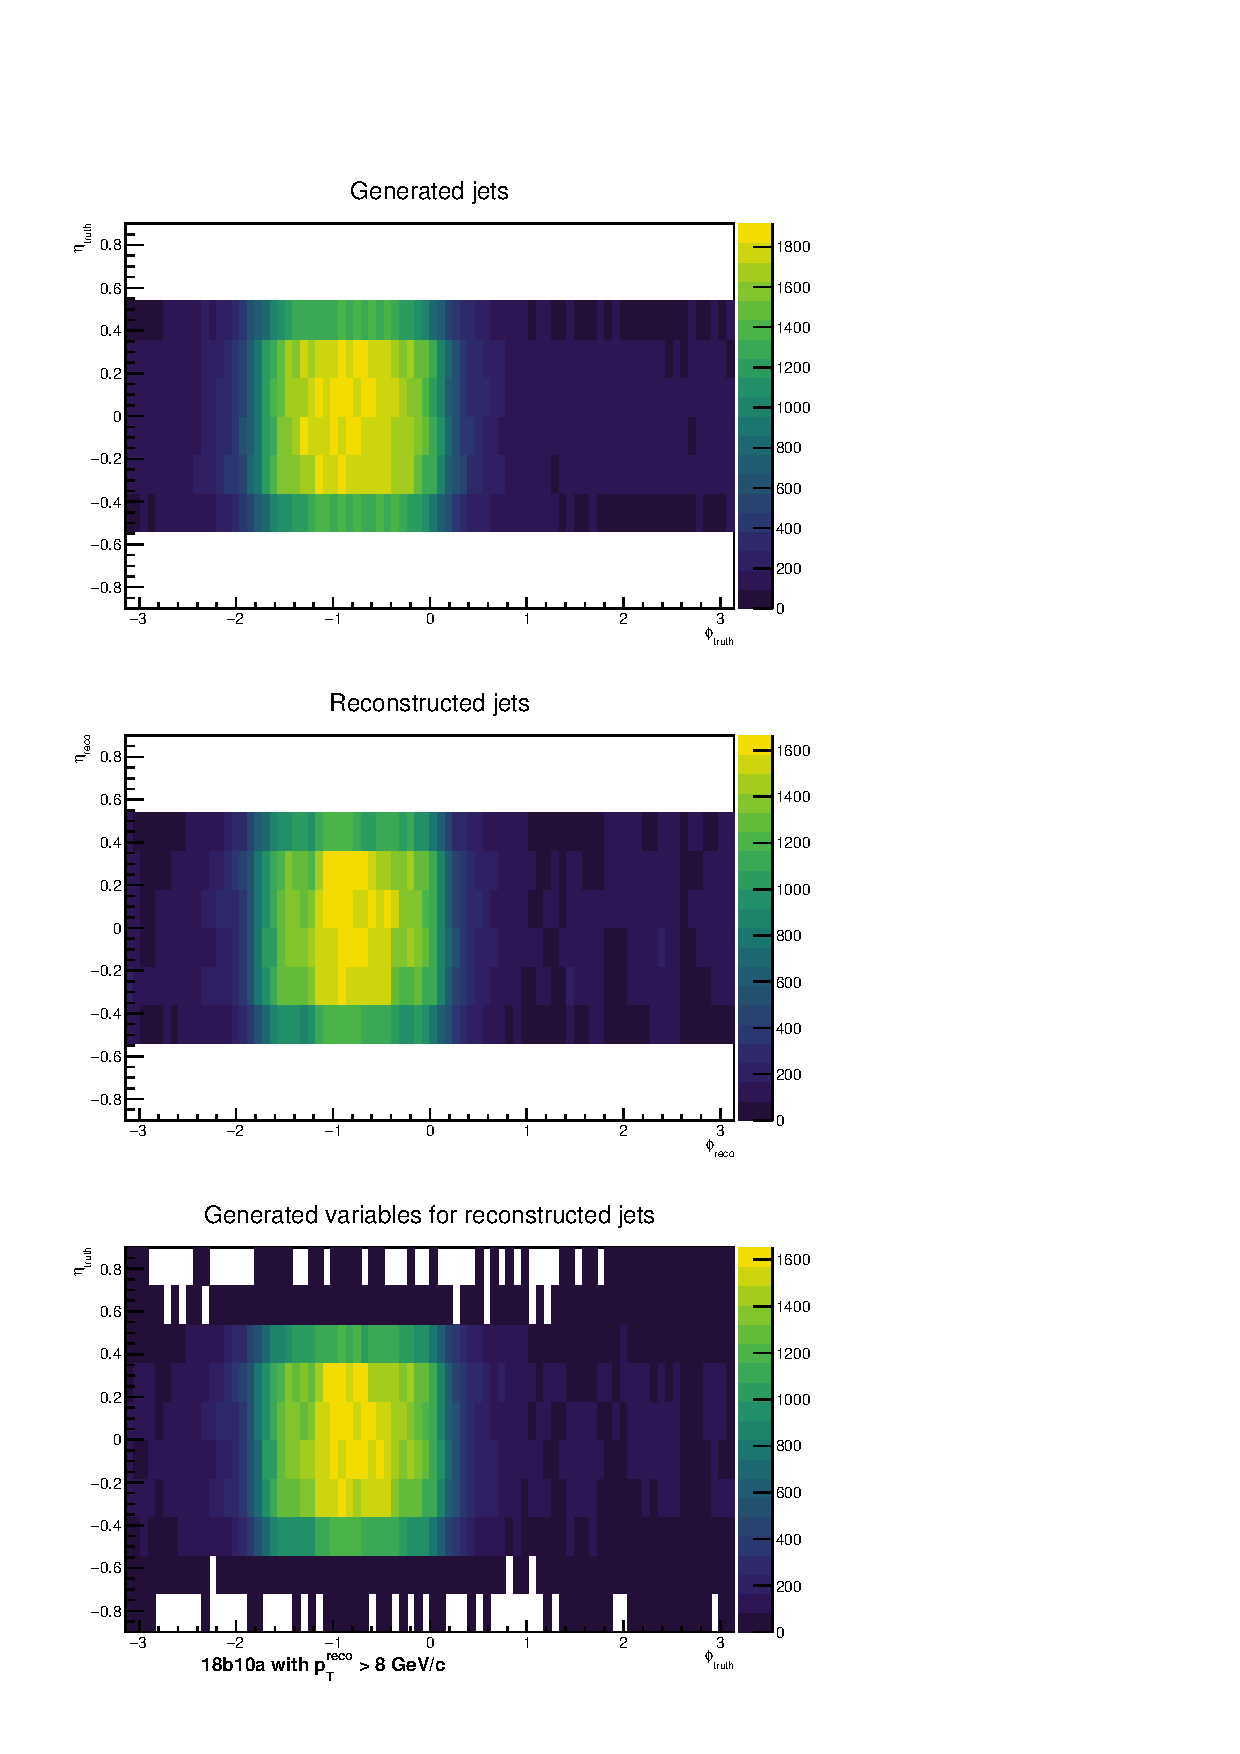
\includegraphics[width=.495\textwidth]{JetResponse/jets_etaPhi_its_pp.pdf}
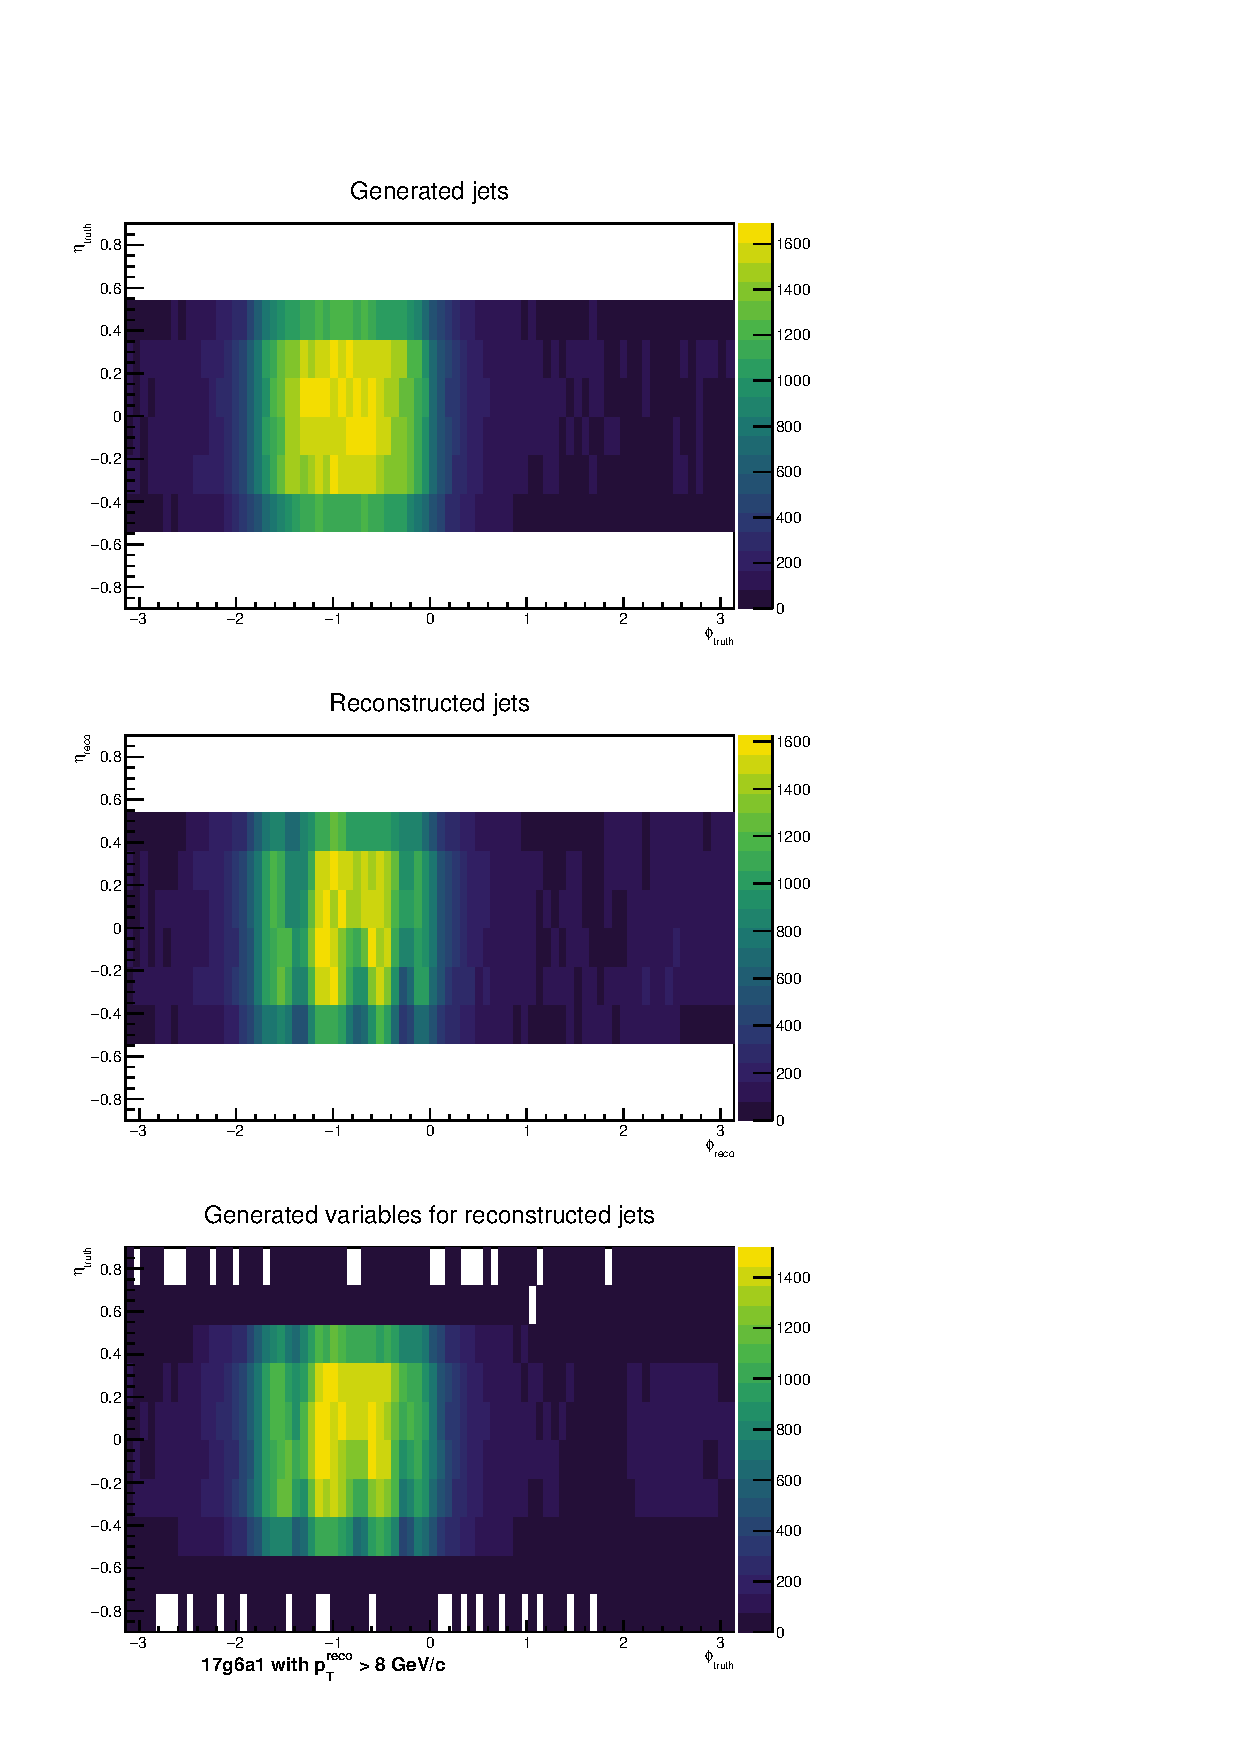
\includegraphics[width=.495\textwidth]{JetResponse/jets_etaPhi_its_pPb.pdf}
\caption{The $\eta$ and $\phi$ distribution of jets in pp (left), and p-Pb (right). The top row are the generated jets while, the middle row has reconstructed jets. The bottom row has the generated variables for the reconstructed jets, so there is a 1-to-1 correspondence between each jet in the middle row and the jet in the bottom row.}
\label{fig:2Djets}
\end{figure}

Figure~\ref{fig:2DEffjets} shows the efficiency of the ITS in position of the jet. Again, there are visible dips $\phi$ for the p-Pb case, while the pp efficiency is uniform in the signal region ($-$2 rad $< \phi <$ 0.5 rad). The efficiency is calculated in a similar manner to the $\eta$ and $\phi$ efficiency for tracking, using equation~\ref{eq:eff}, but as a function of $\eta$ and $\phi$ instead of the \pt.  
\begin{figure}[h]
\center
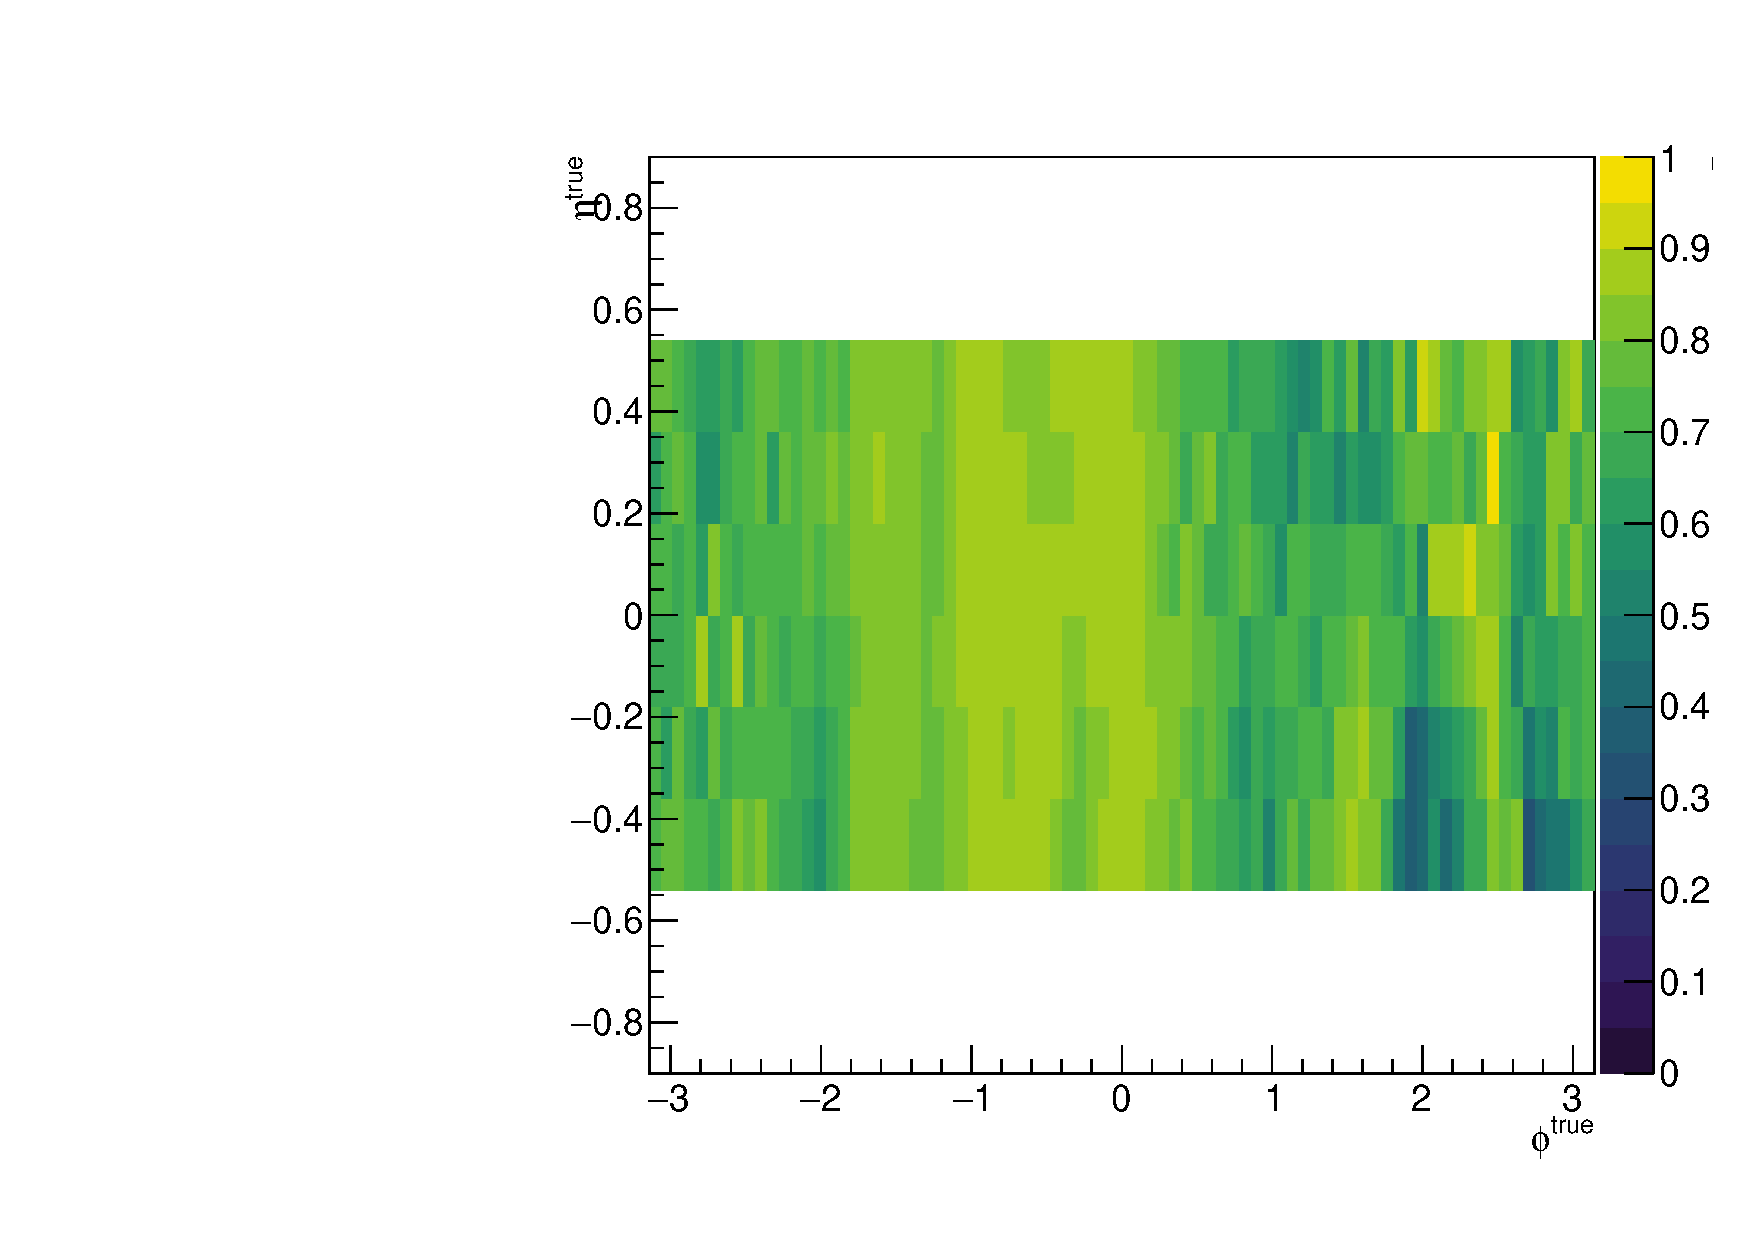
\includegraphics[width=.495\textwidth]{JetResponse/jet_etaPhi_eff_its_pp.pdf}
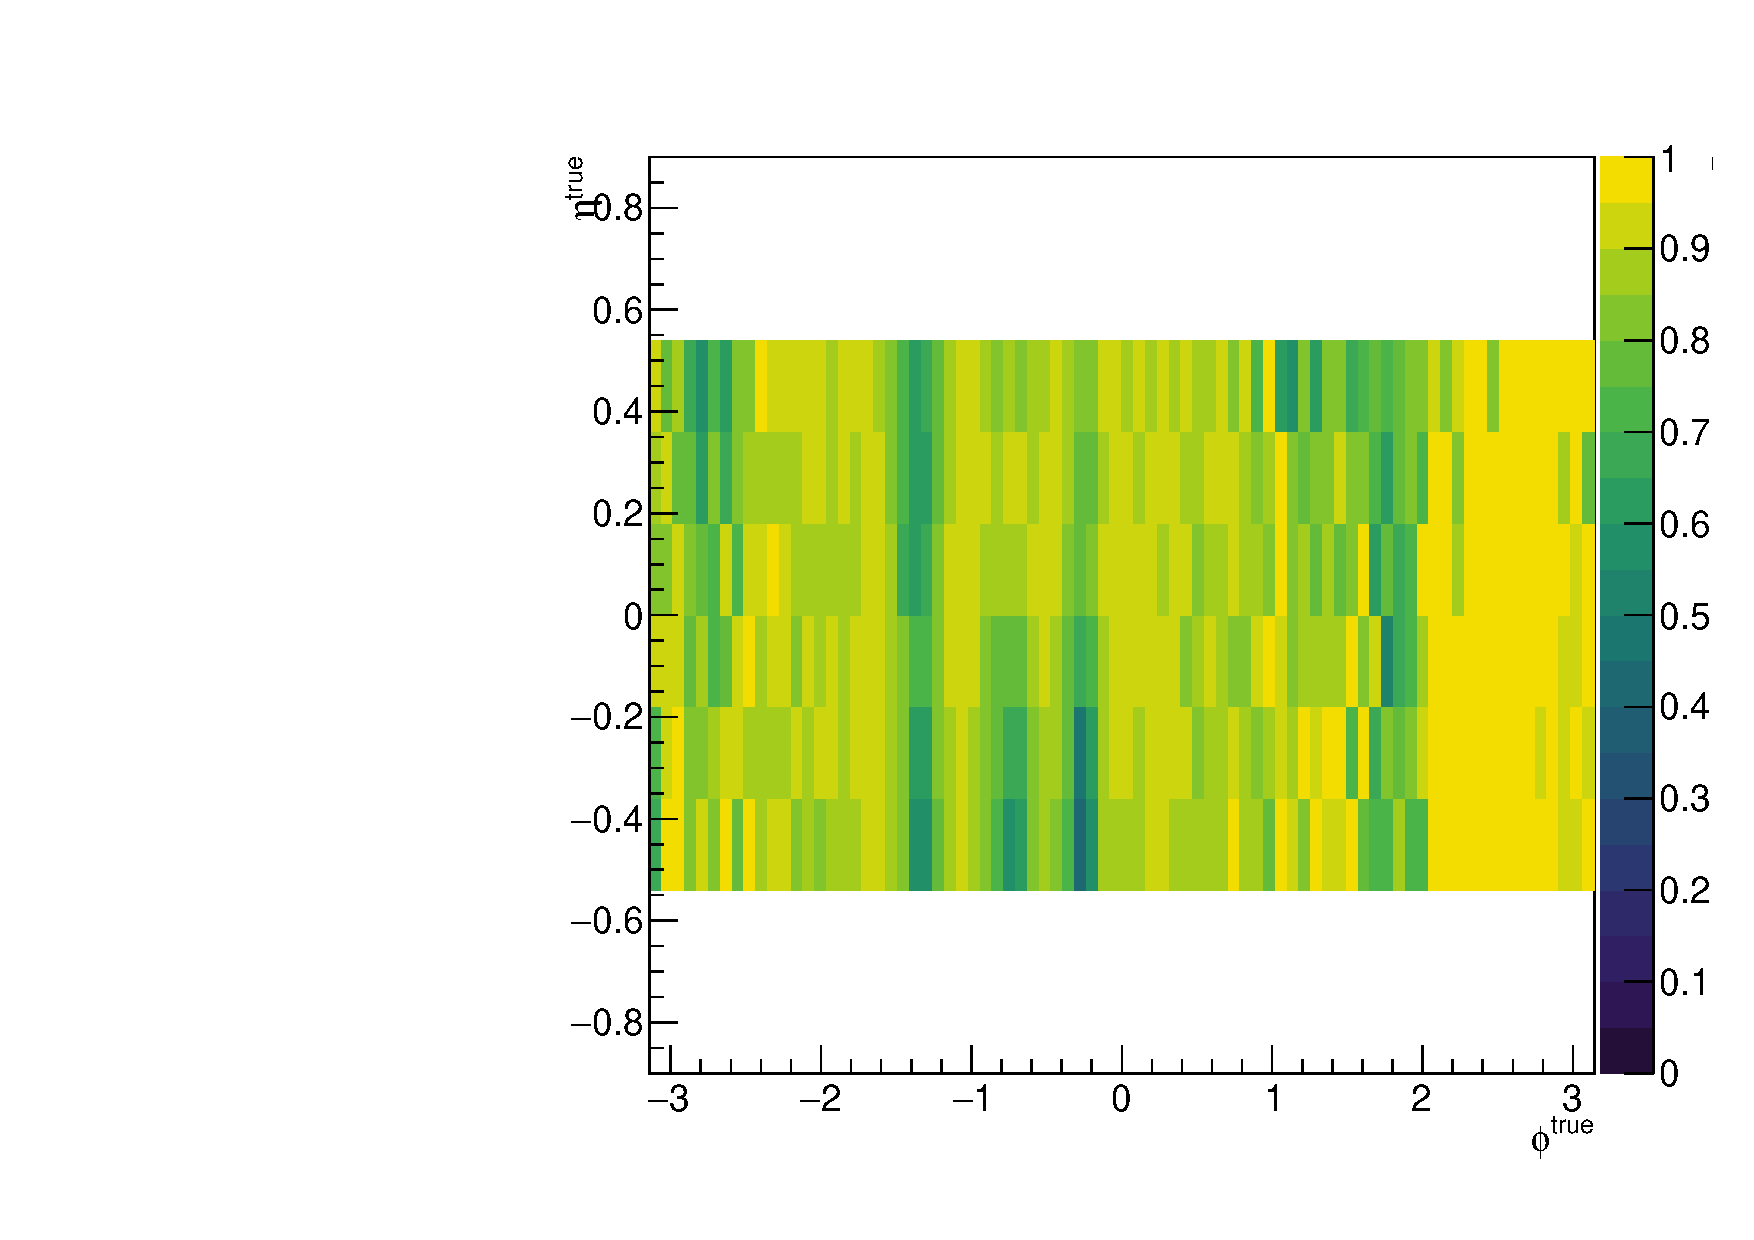
\includegraphics[width=.495\textwidth]{JetResponse/jet_etaPhi_eff_its_pPb.pdf}
\caption{The $\eta$ and $\phi$ efficiency for pp (left) and p-Pb (right). The efficiency is calculated as the ratio of generated truth and reconstructed truth variables, using LHC17g6a1 and LHC18b10a for p-Pb and pp respectively.}
\label{fig:2DEffjets}
\end{figure}

Figure~\ref{fig:2DSmearjets} shows the smearing effects to due to the tracking resolution of ITS only tracking. The smearing effect is calculated as the ratio of MC truth and MC reco for reconstructed jets. The fact that the ratio close to one implies that we do not see very large smearing effects.  
\begin{figure}[h]
\center
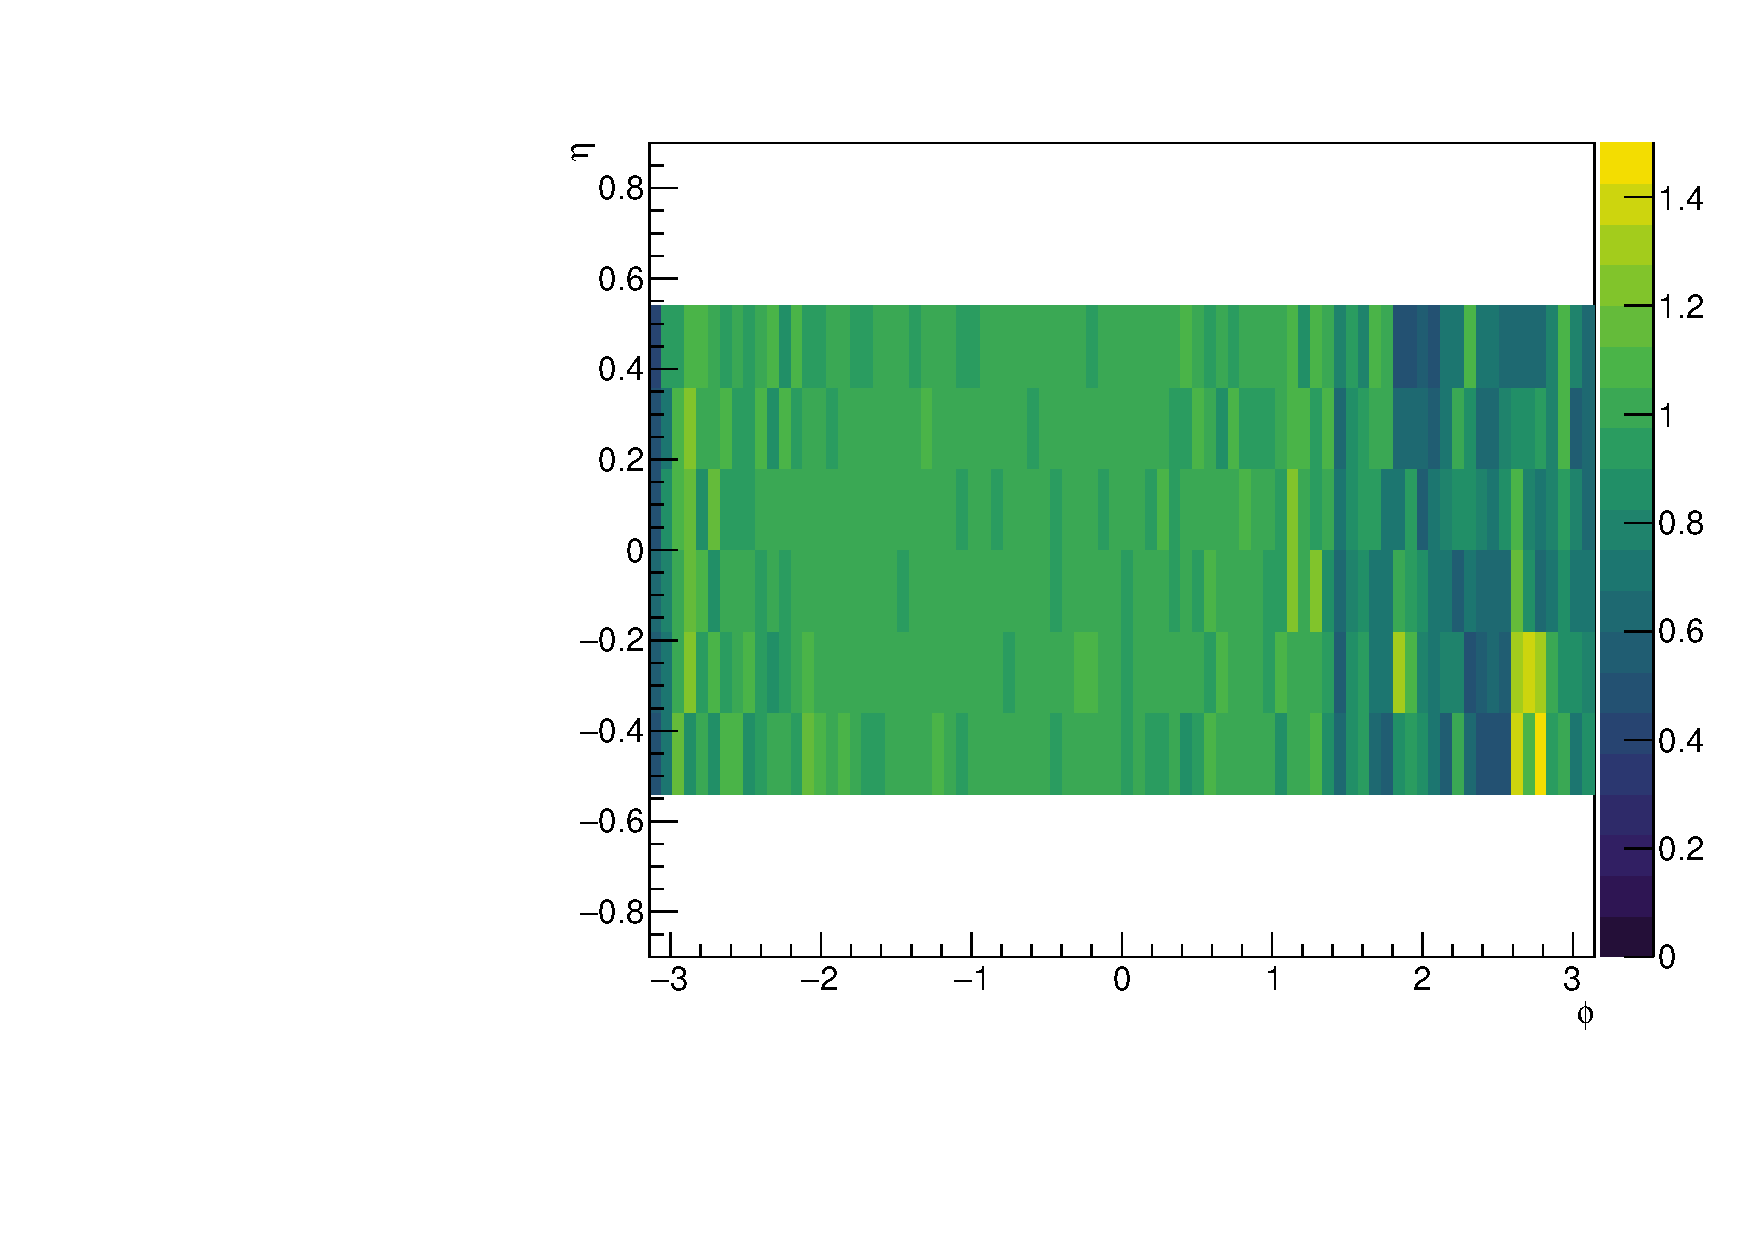
\includegraphics[width=.495\textwidth]{JetResponse/jet_etaPhi_BinbyBin_its_pp.pdf}
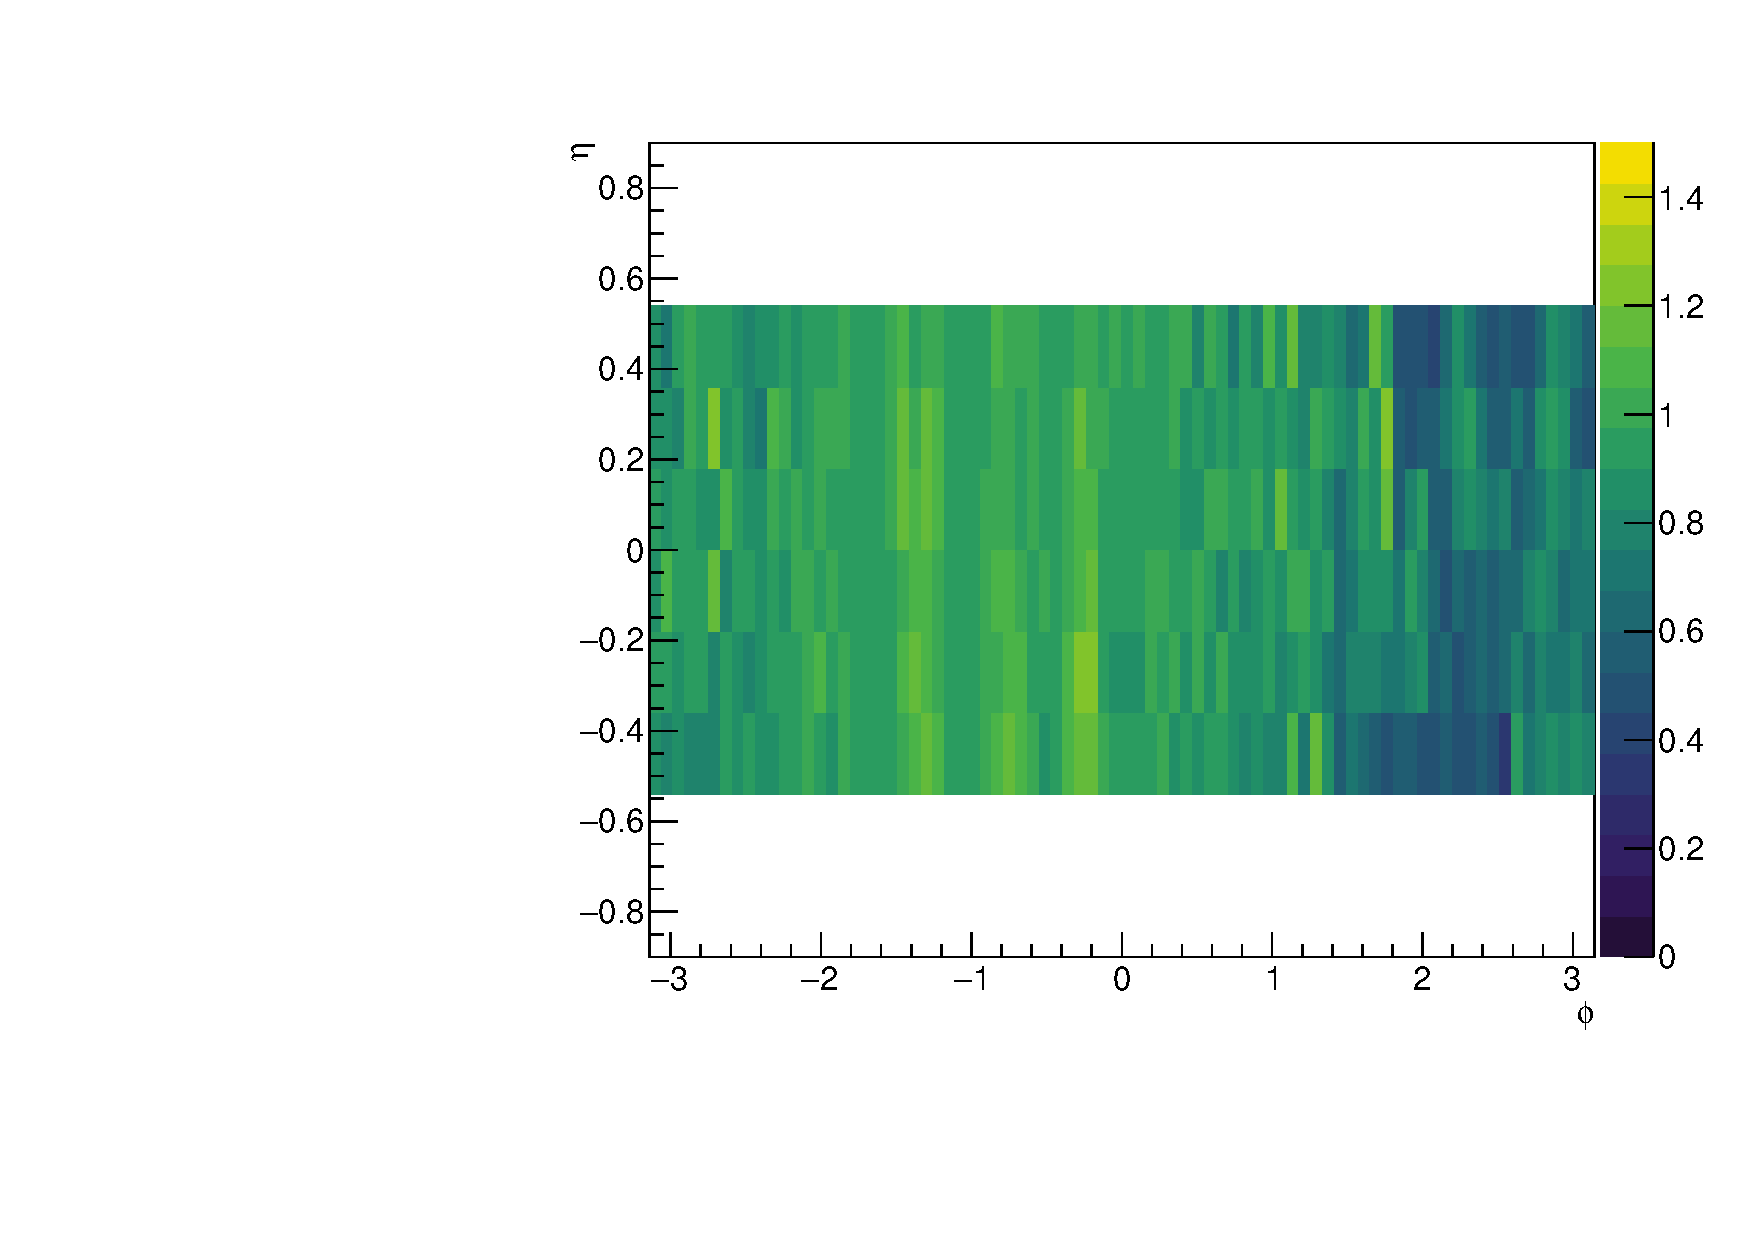
\includegraphics[width=.495\textwidth]{JetResponse/jet_etaPhi_BinbyBin_its_pPb.pdf}
\caption{The $\eta$ and $\phi$ distribution of the smearing effect between the truth and reconstructed variables of reconstructed jets for pp (left) and p-Pb (right), using LHC17g6a1 and LHC18b10a for p-Pb and pp respectively.}
\label{fig:2DSmearjets}
\end{figure}

\subsection{Azimuthal angular dependence pf the Jet Response}
Figure~\ref{fig:jetphi} is a projection of figure~\ref{fig:2Djets} on the $\phi$ axis. It shows the $\phi$ distribution of jets. Again, the peak is due the fact that these are recoil jets opposite to photons in the EMCal. We can see that the truth (blue) and reconstructed (red) variables for reconstructed jets match quite well. There is a different of 3\% between the integral of the two histograms, which implies that 3\% of reconstructed jets do not have a matching true jet. Additionally, the dips due the holes in the ITS are seen in p-Pb distribution. 

\begin{figure}[h]
\center
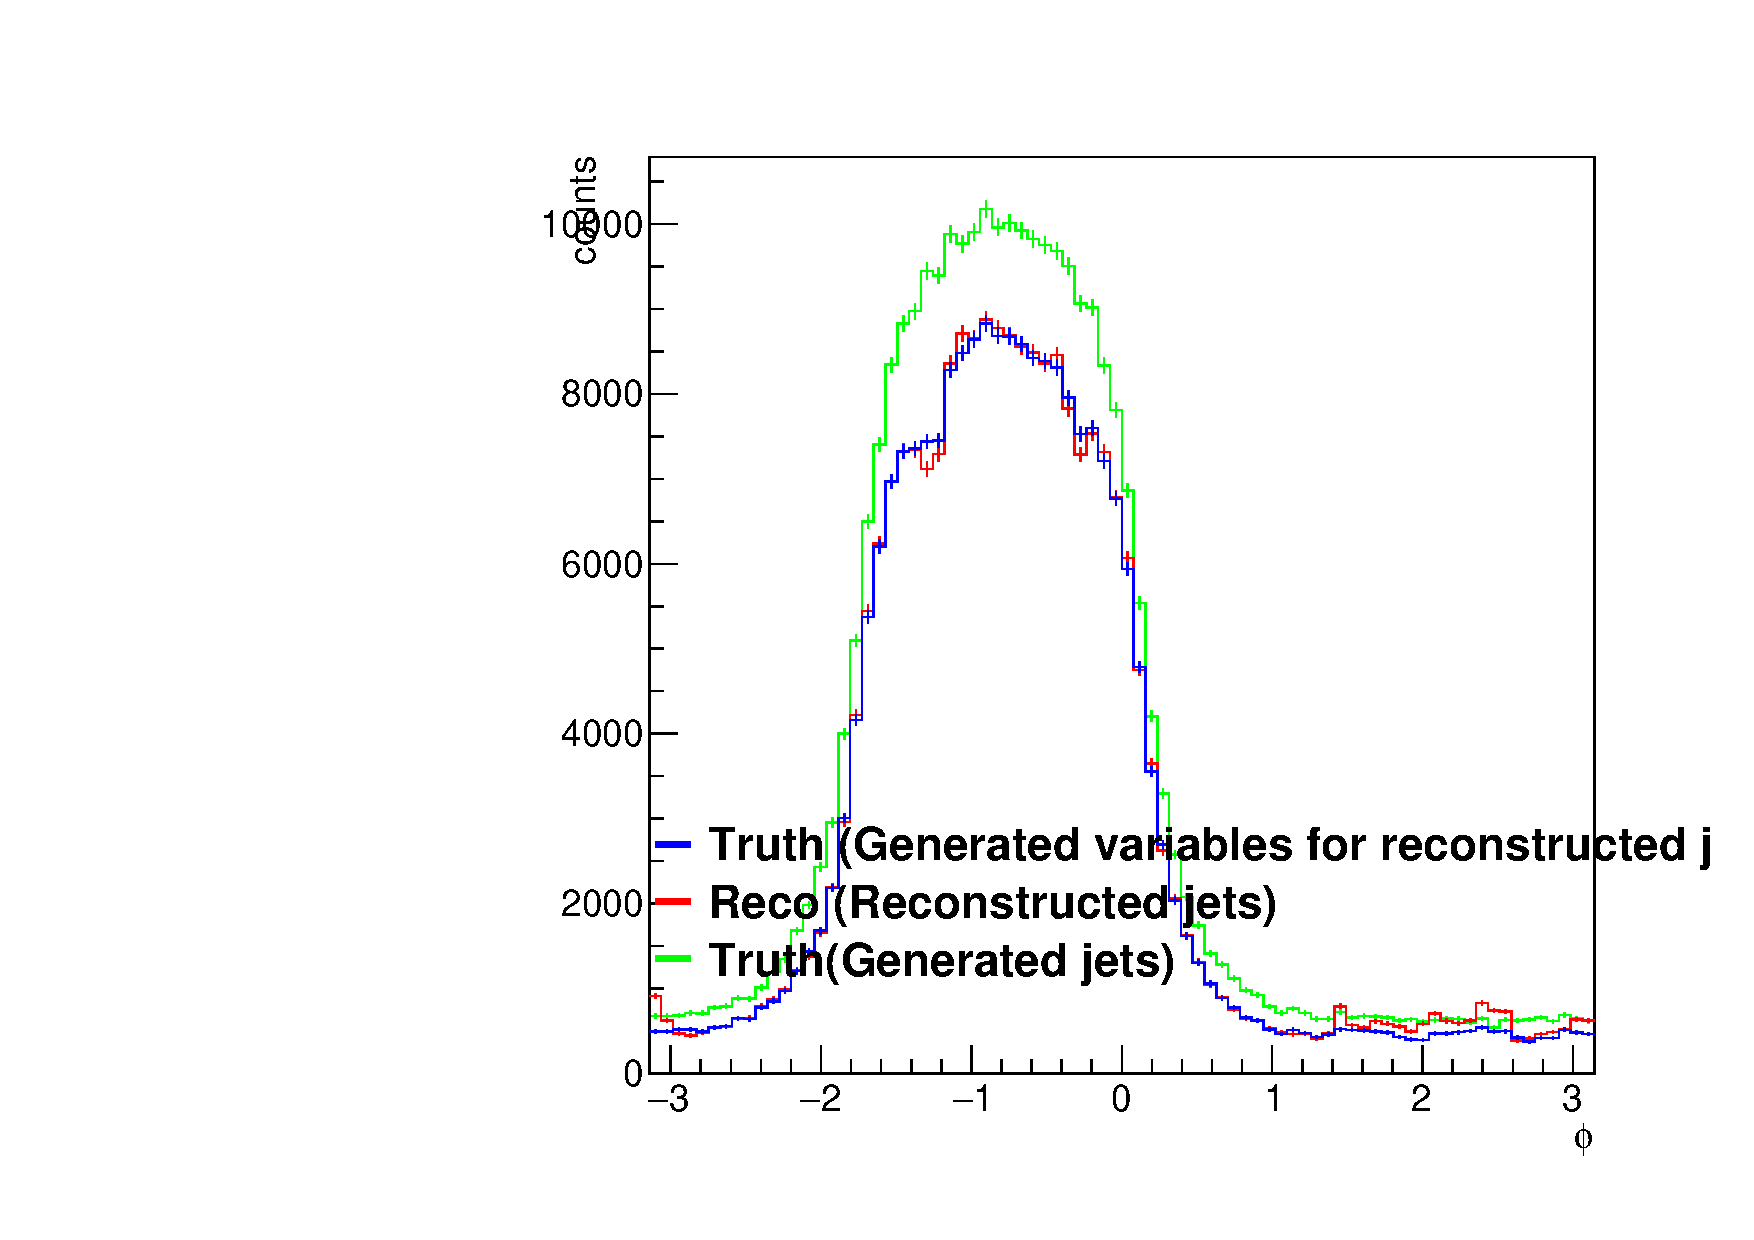
\includegraphics[width=.495\textwidth]{JetResponse/jet_phi_distribution_pp_8GeV.pdf}
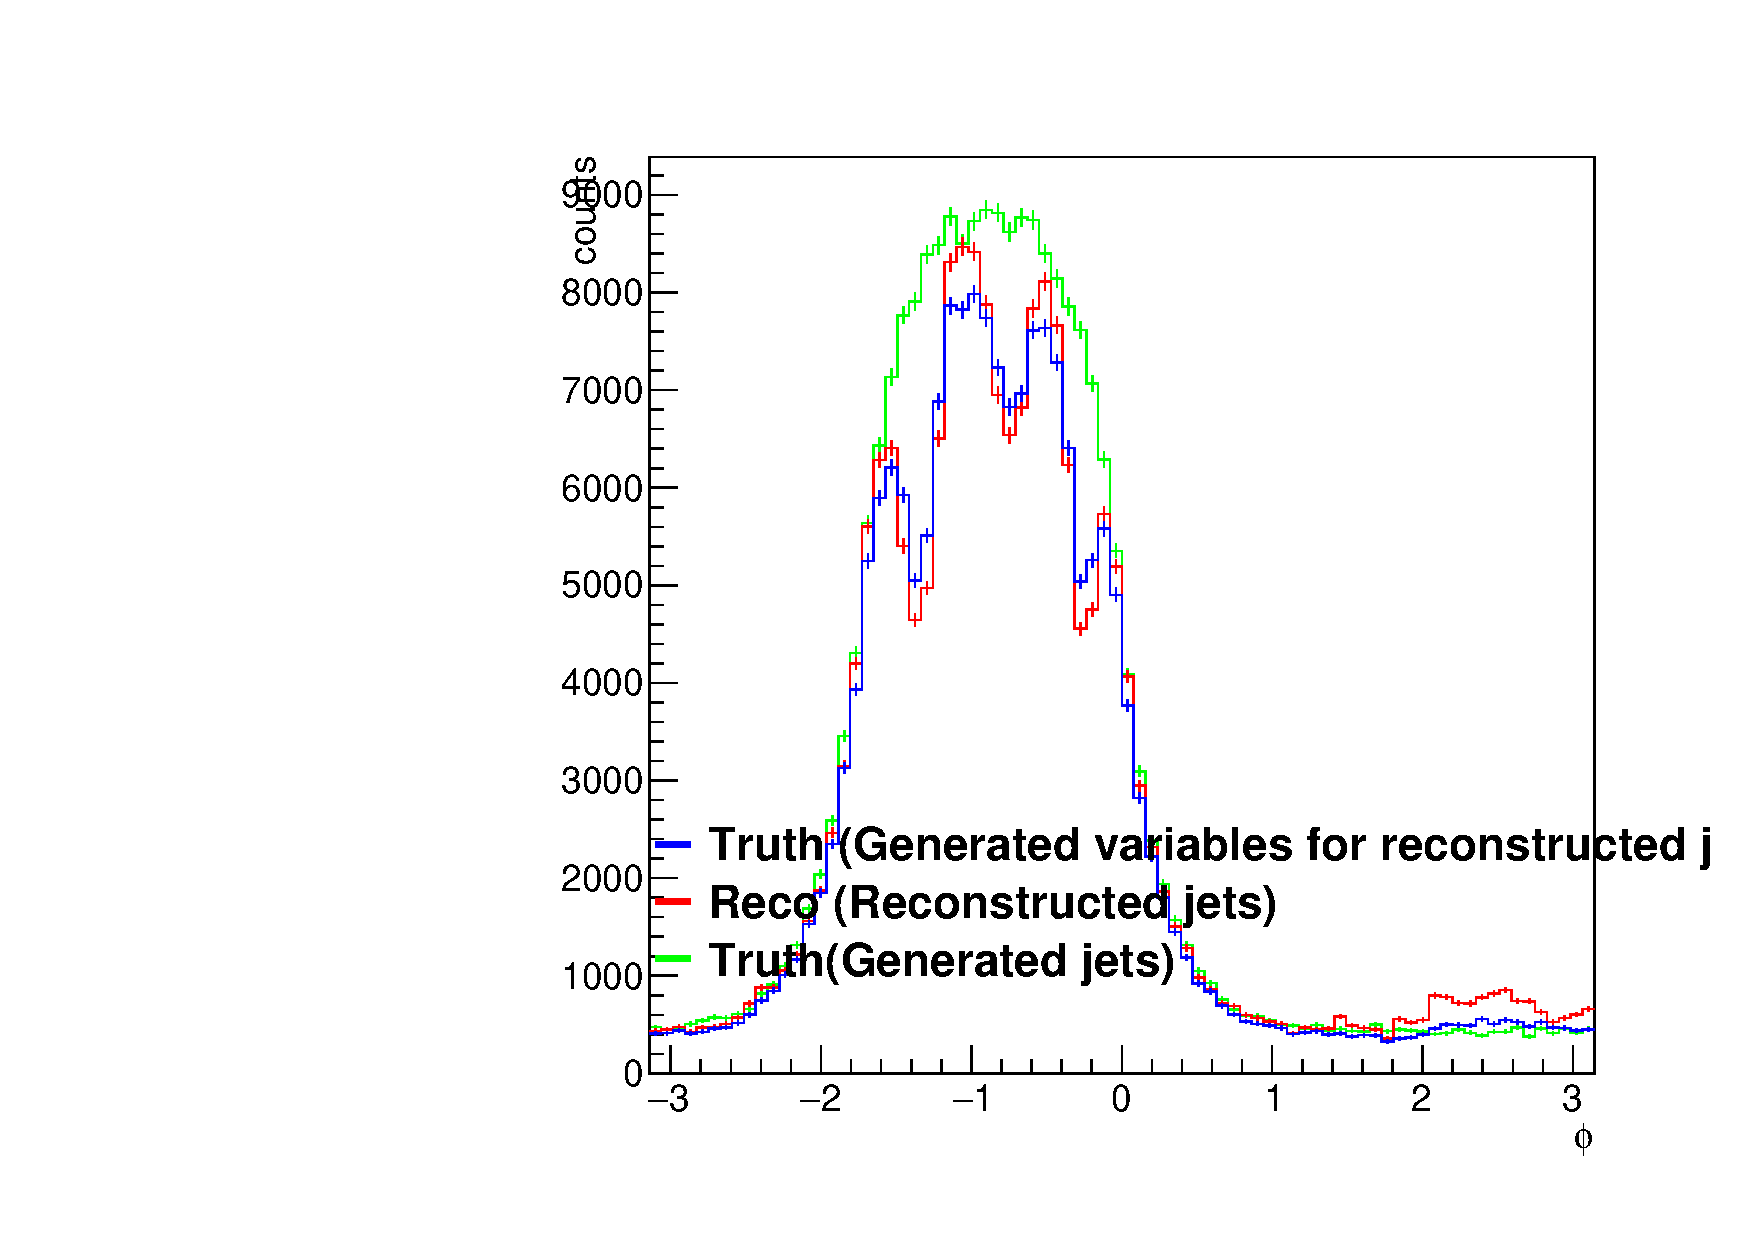
\includegraphics[width=.495\textwidth]{JetResponse/jet_phi_distribution_pPb_8GeV.pdf}
\caption{The $\phi$ distribution of jets in pp (left), and p-Pb (right), using LHC17g6a1 and LHC18b10a for p-Pb and pp respectively. The peak is due to the fact that these are recoil jets opposite to a photon in the EMCal. The effect to due the holes in ITS is present in p-Pb, but not in pp as they were fixed for the pp period.}
\label{fig:jetphi}
\end{figure}

%Figure~\ref{fig:jetphiEff} is the efficiency as function of $\phi$. The efficiency is calculated using equation~\ref{eq:eff}, but as a function of $\phi$. It is a the ratio of the blue distribution divide by the green distribution from figure~\ref{fig:jetphi}. The dips due to the holes are clearly visible in the p-Pb efficiency, while, we a almost uniform distribution for the pp efficiency in signal region.
%\begin{figure}[h]
%\center
%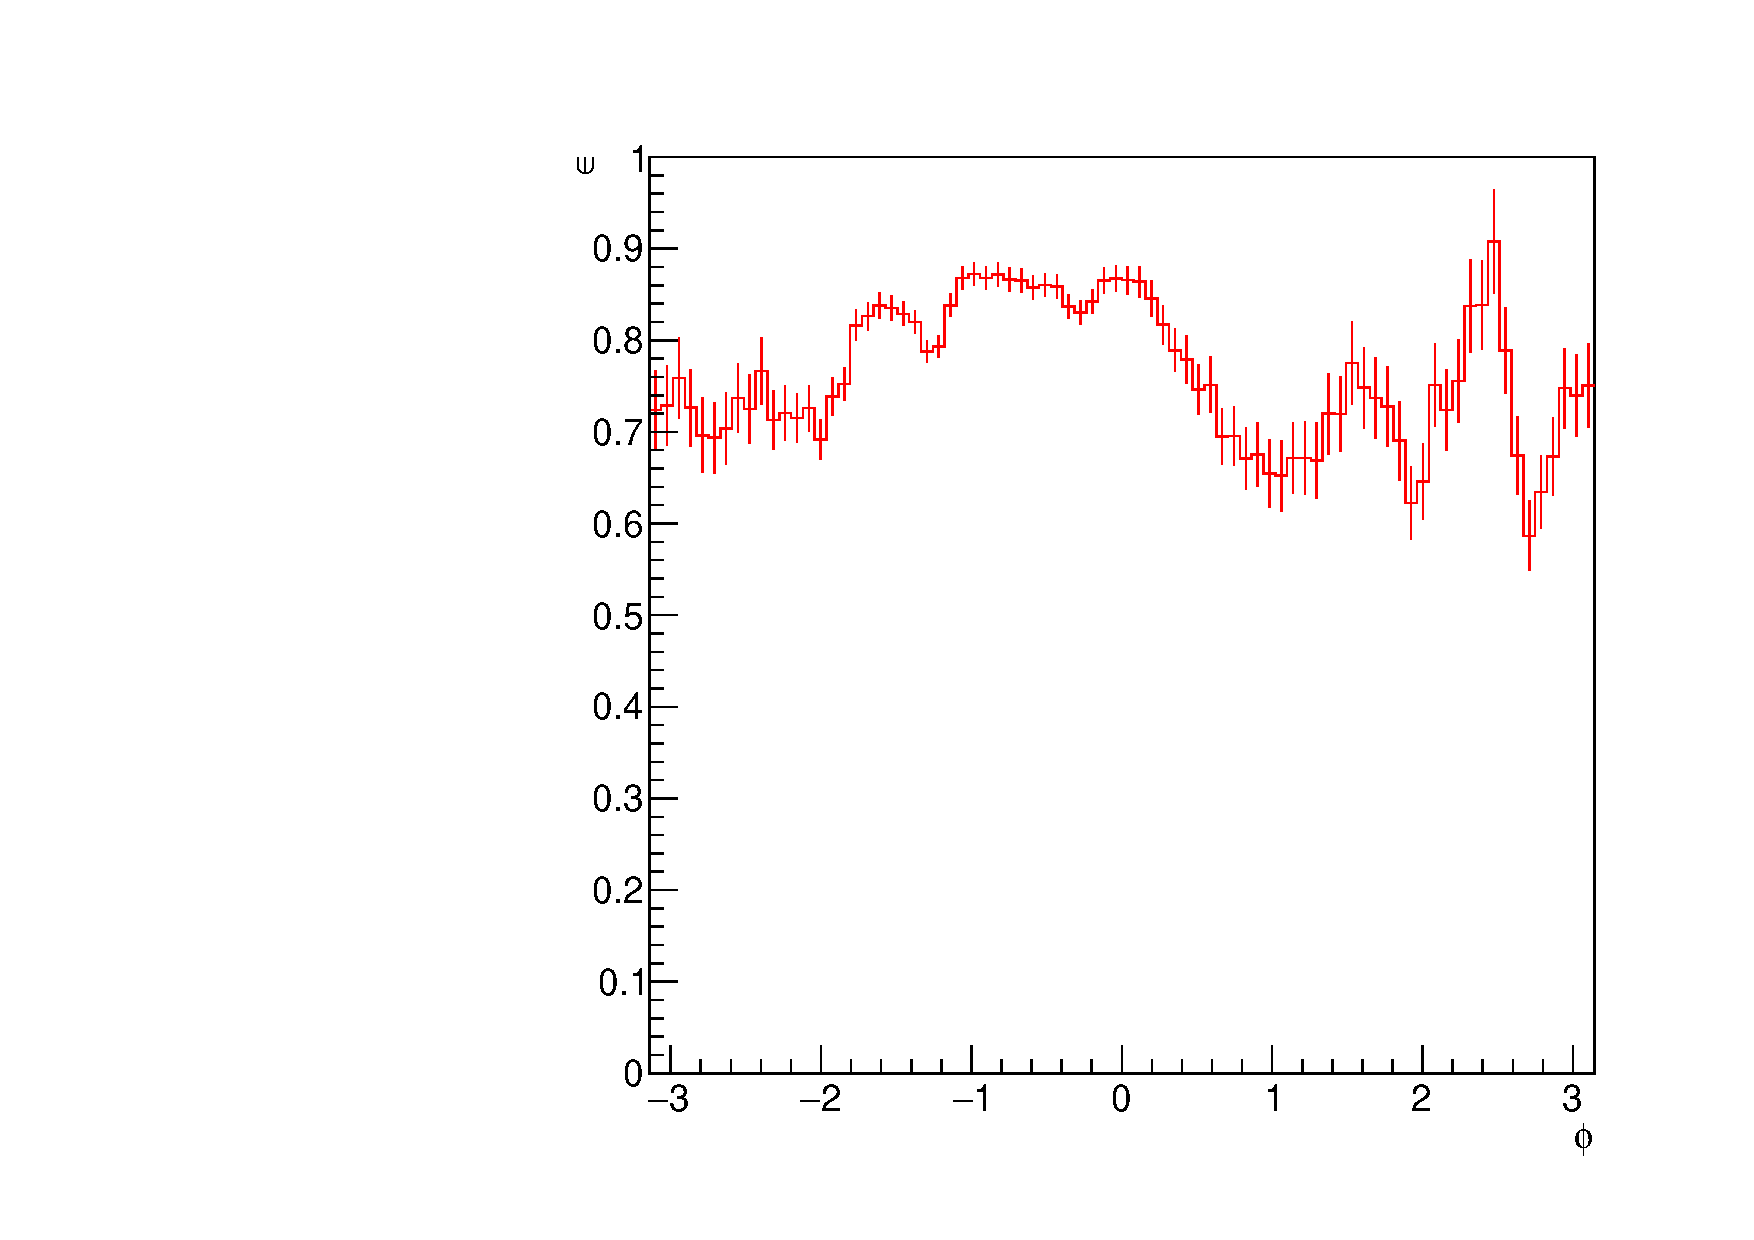
\includegraphics[width=.495\textwidth]{JetResponse/jet_phiEff_its_pp.pdf}
%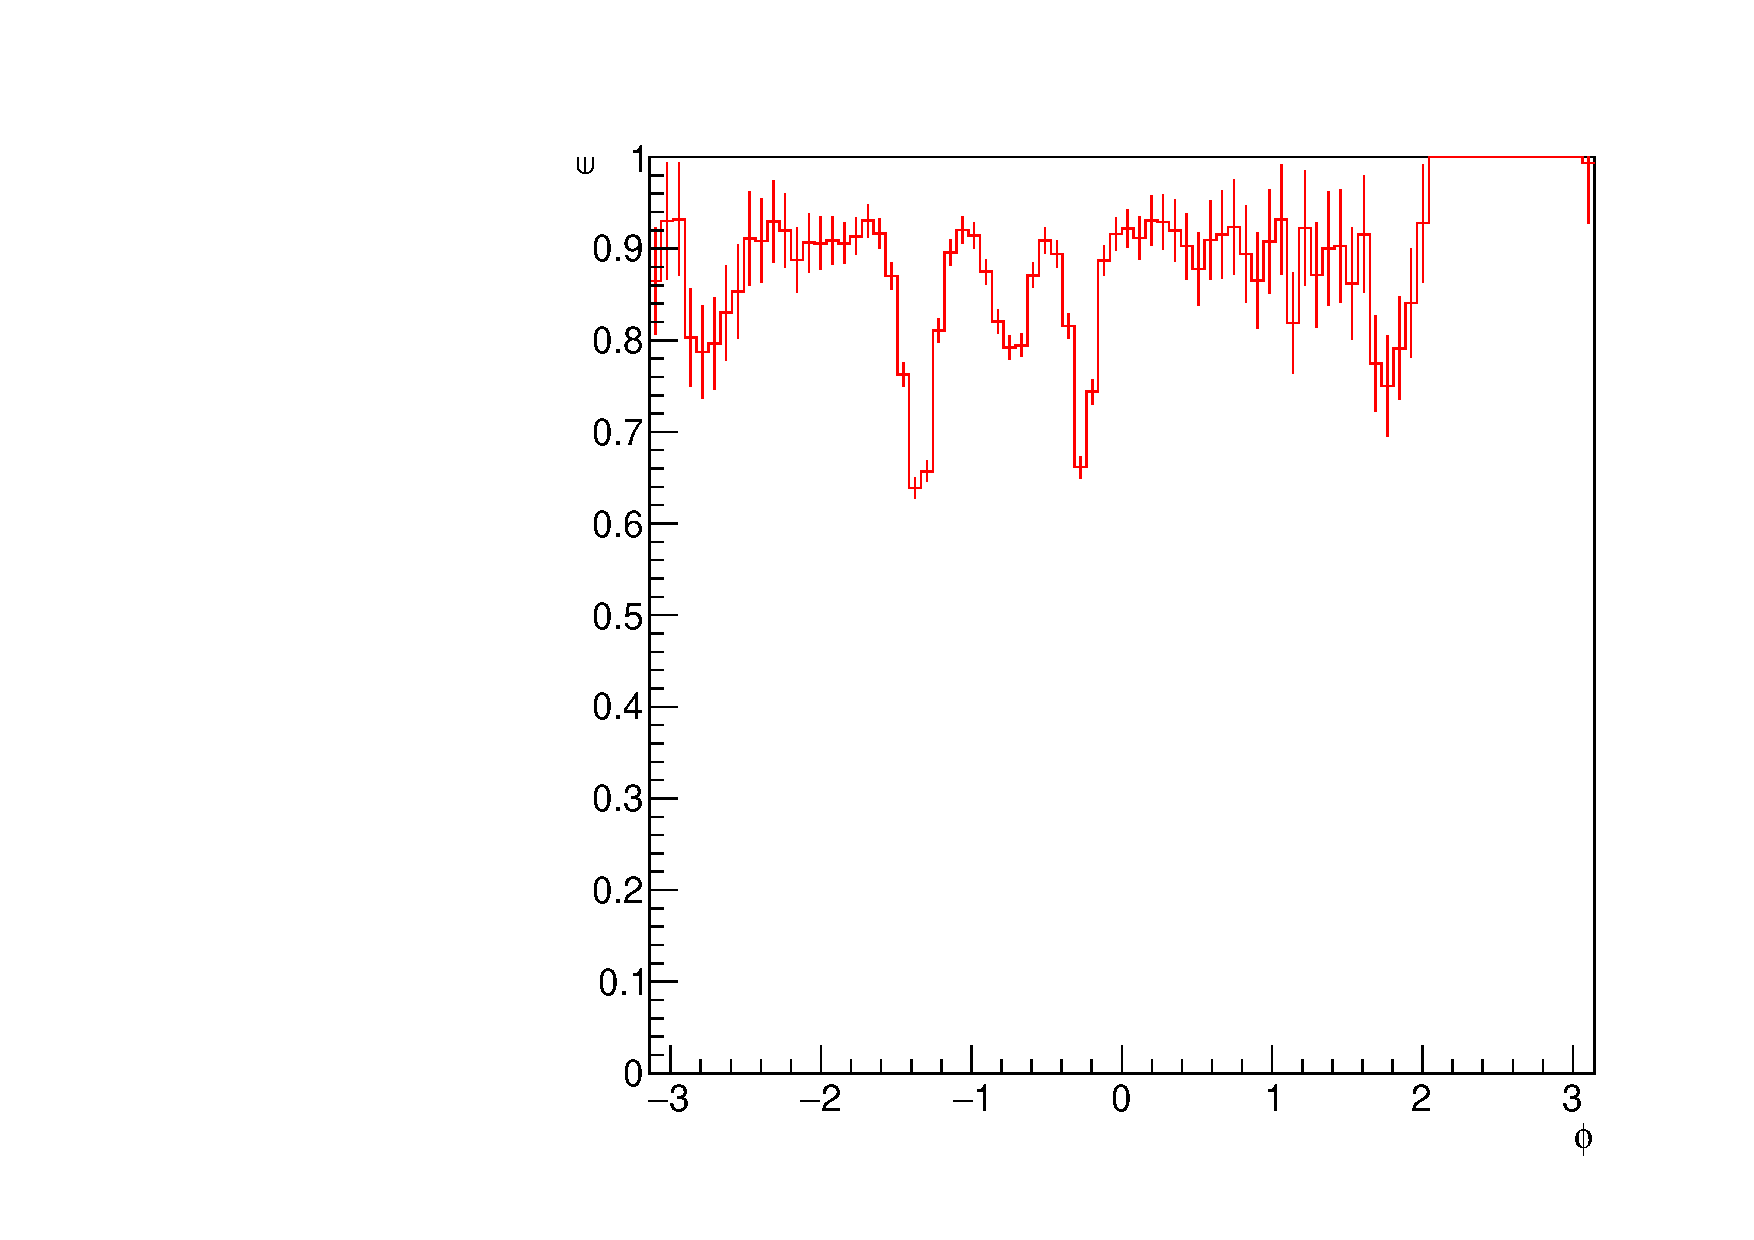
\includegraphics[width=.495\textwidth]{JetResponse/jet_phiEff_its_pPb.pdf}
%\caption{The $\phi$ efficiency of jets in pp (left), and p-Pb (right), using LHC17g6a1 and LHC18b10a for p-Pb and pp respectively. The efficiency loss due to the holes in the ITS is visible in the p-Pb plot at $\phi = -1.2$ and $-$0.2.}
%\label{fig:jetphiEff}
%\end{figure}

Figure~\ref{fig:jetphidphiRes} shows detector resolution in azimuth, as a function of $\phi^{\mathrm{true}}$, for jets. The resolution is the spread in the difference between truth $\phi$ and reconstructed $\phi$ for a reconstructed jet, and we can see that, detector resolution is very good and there is not a strong deviation from 0.0 in either pp or p-Pb. 85\% of the statistics for pp and and 92\% of the statistics for p-Pb lie within -0.02 $< \Delta\phi <$ 0.02. 
\begin{figure}[h]
\center
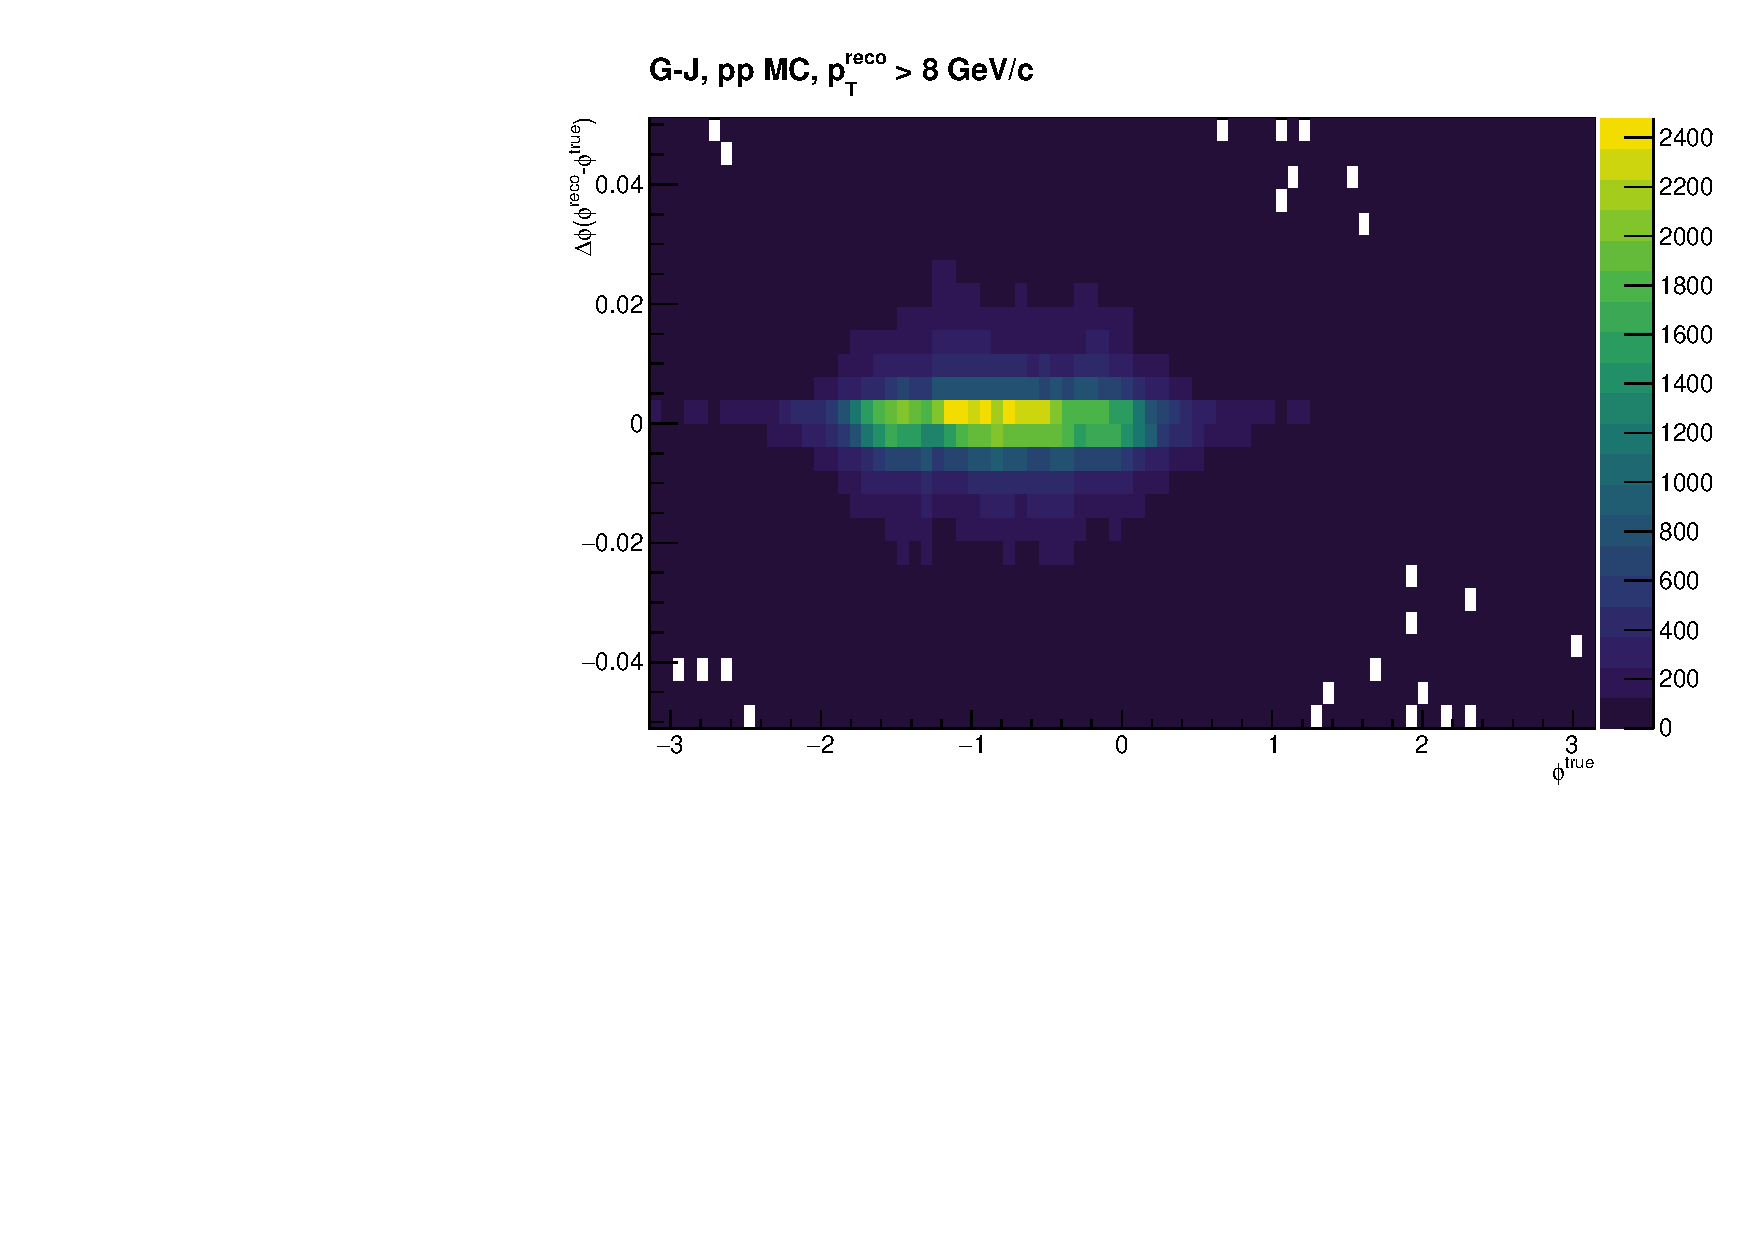
\includegraphics[width=.495\textwidth]{JetResponse/dphivphi_pp.pdf}
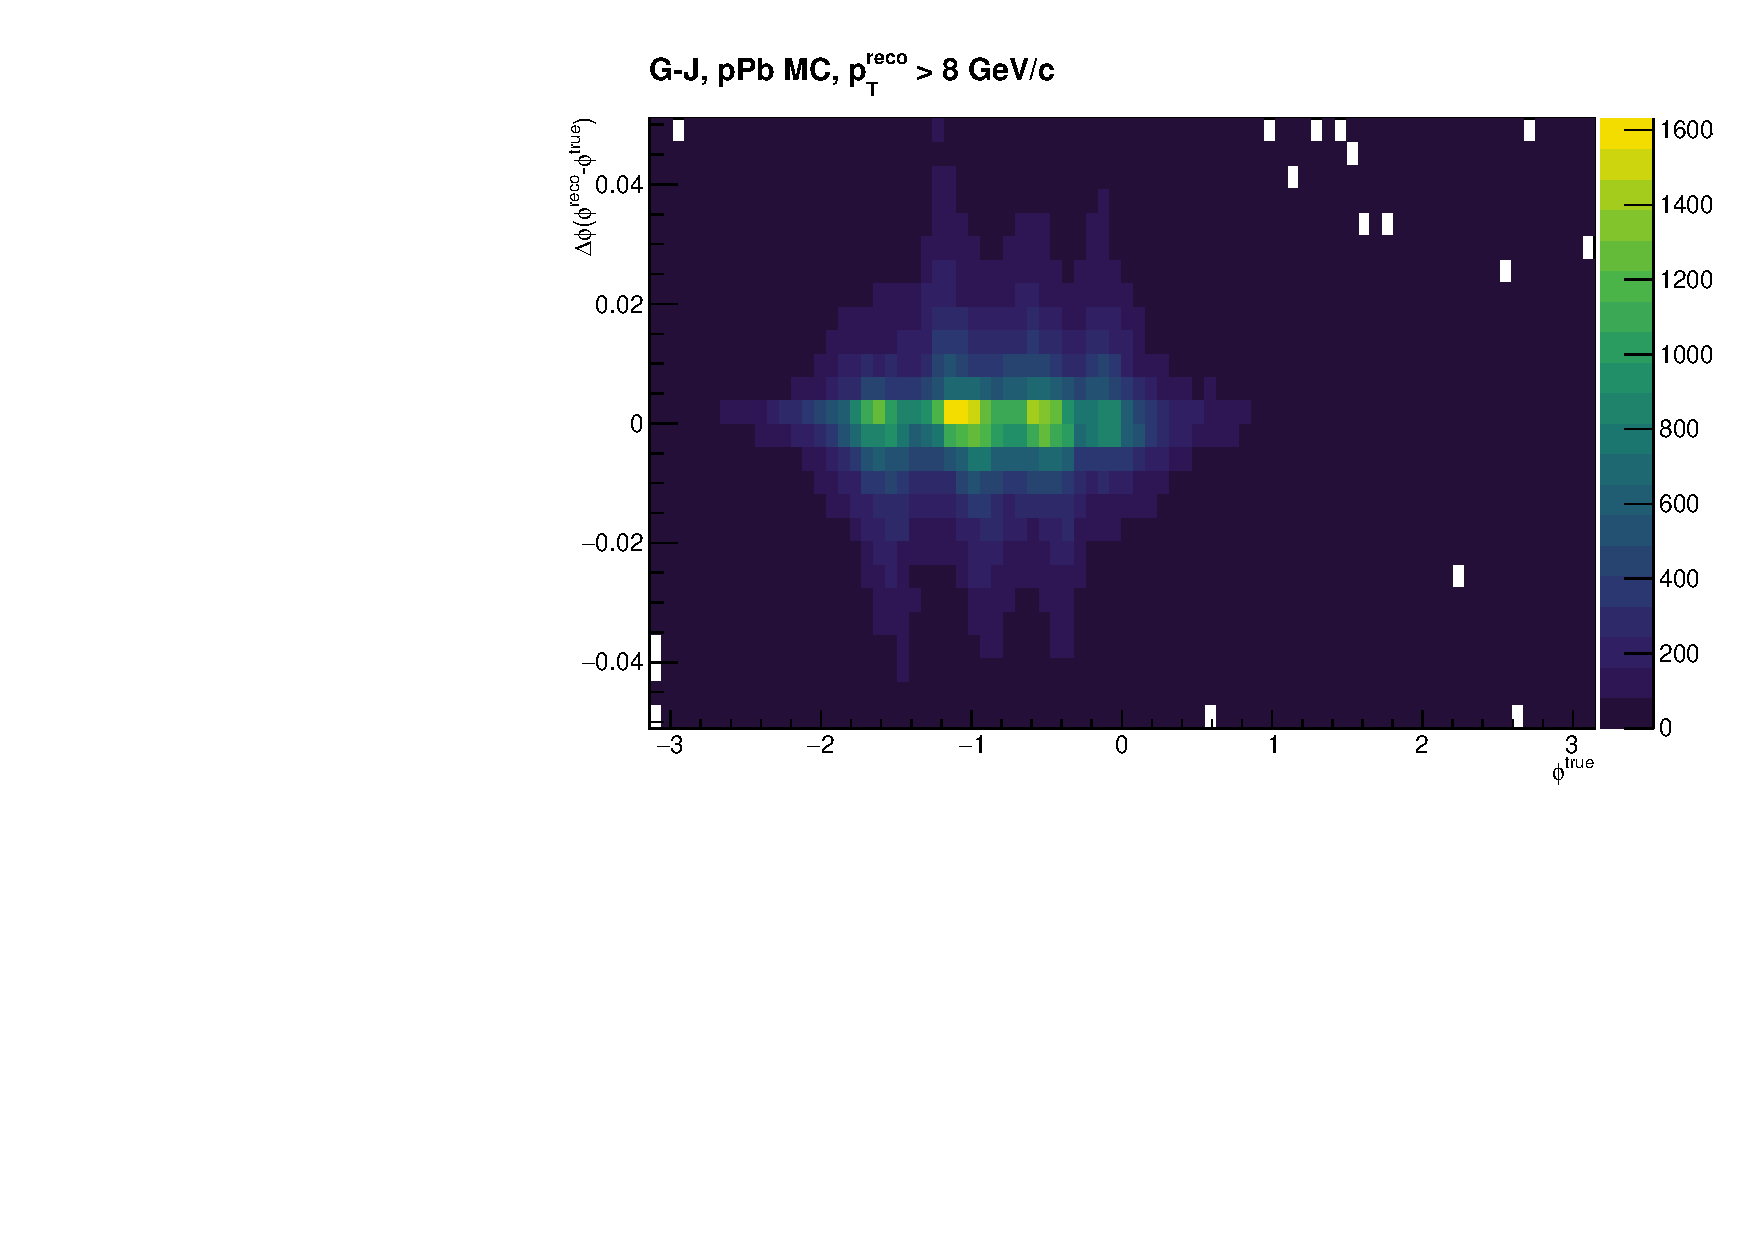
\includegraphics[width=.495\textwidth]{JetResponse/dphivphi_pPb.pdf}
\caption{The $\phi$ resolution as a function of $\phi^{true}$ of jets in pp (left), and pPb (right), using LHC17g6a1 and LHC18b10a for p-Pb and pp respectively. The distribution is spread very closely around 0.0, with 78\% and 66\% of the statistics lying in within the band $-$0.01 rad $< \Delta\phi <$ 0.01 rad for pp and pPb respectively. The statistics are concentrated in the region $-$2 rad $< \phi^{\mathrm{true}} <$-0.5 rad because these are recoil jets opposite to a photon in the EMCal acceptance.}
\label{fig:jetphidphiRes}
\end{figure}


Figure~\ref{fig:jetdphiRes} shows the projections of figure~\ref{fig:jetphidphiRes} on to the $\Delta\phi$ axis. The $\phi$ resolution peaks at zero, and has a root mean square of 0.01 and 0.02 for pp and p-Pb respectively. This indicates that the jet resolution in $\phi$ is pretty and does not deviate very much from the true value.
\begin{figure}[h]
\center
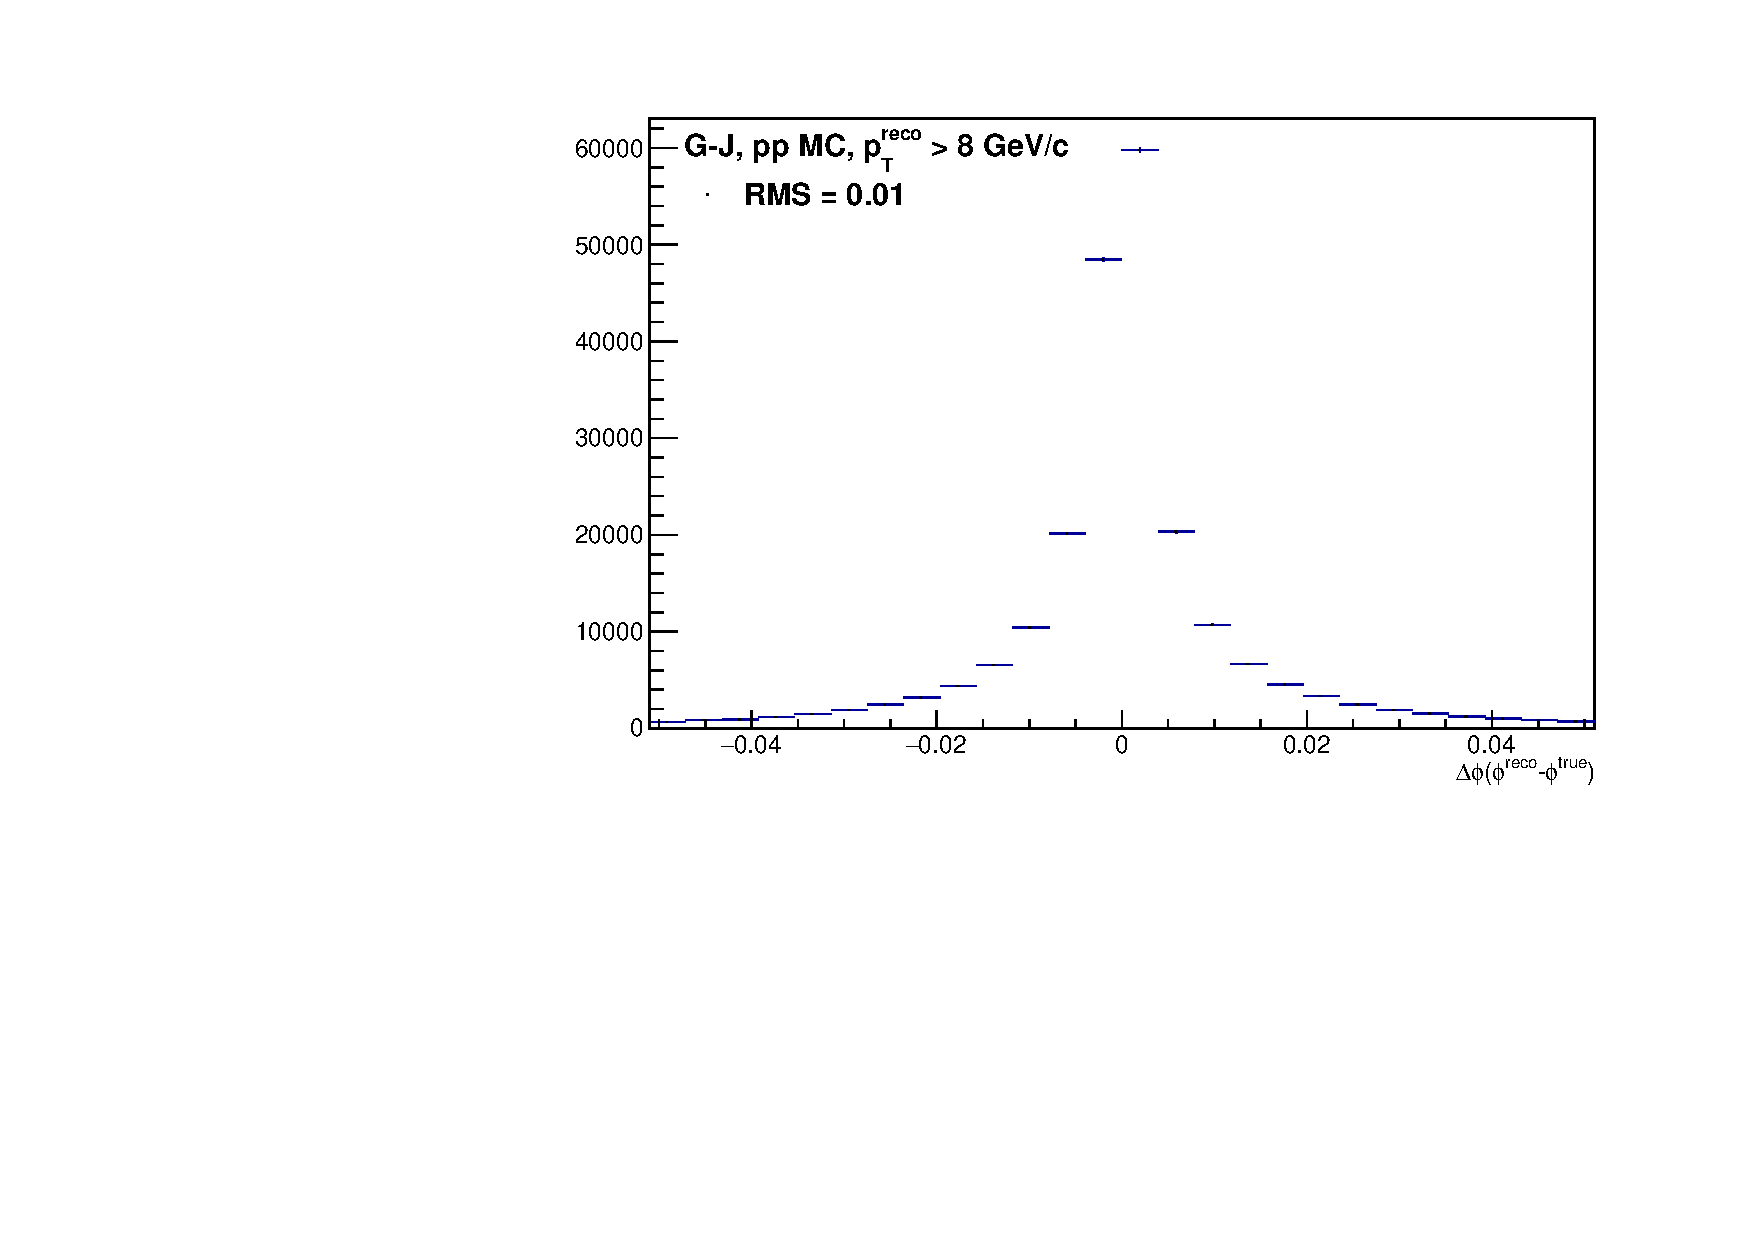
\includegraphics[width=.495\textwidth]{JetResponse/dphi_pp.pdf}
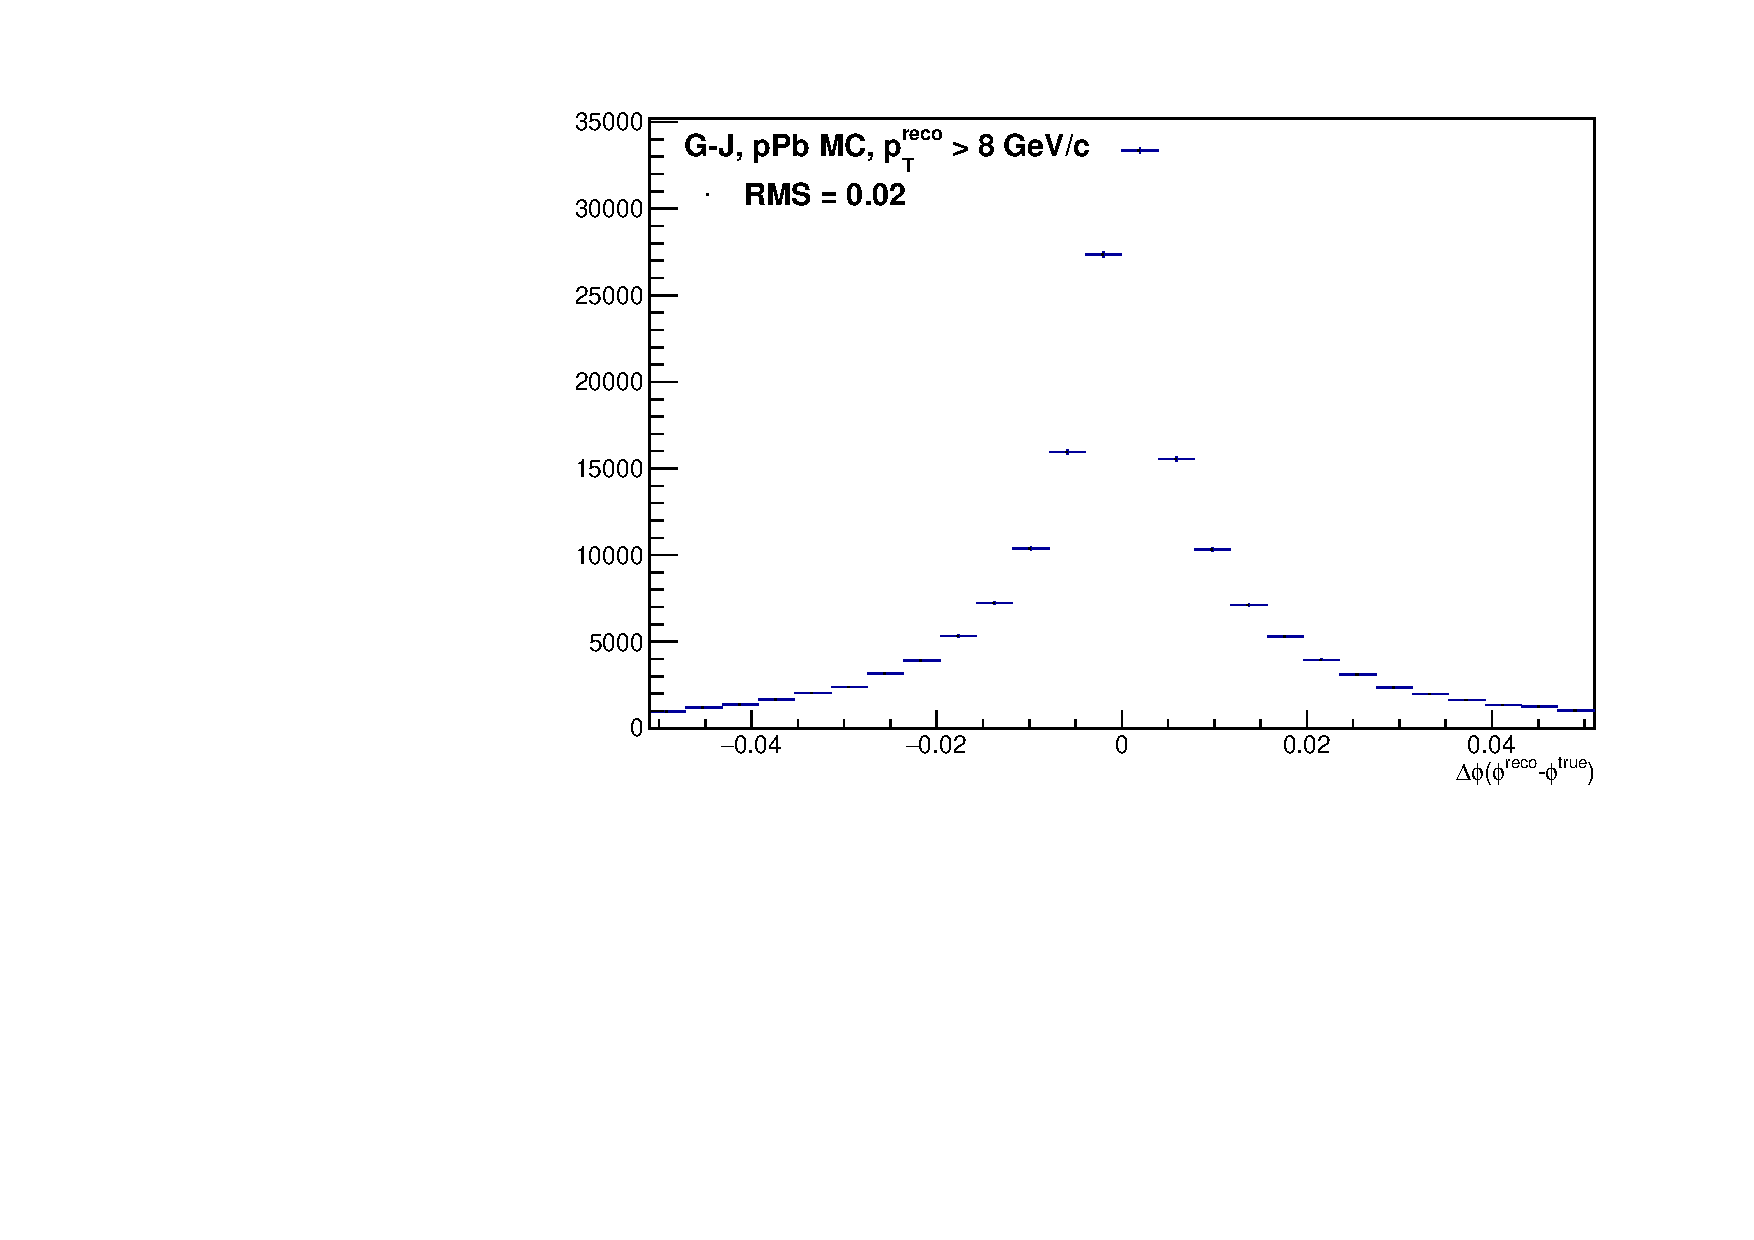
\includegraphics[width=.495\textwidth]{JetResponse/dphi_pPb.pdf}
\caption{The $\phi$ resolution as a function of $\phi^{true}$ of jets in pp (left), and p-Pb (right), using LHC17g6a1 and LHC18b10a for p-Pb and pp respectively. The distribution is spread very closely around 0.0, with 78\% and 66\% of the statistics lying in within the band -0.01 rad $< \Delta\phi <$ 0.01 rad for pp and p-Pb respectively. The statistics are concentrated in the region $-$2 rad $< \phi^{true} <$-0.5 rad because these are recoil jets opposite to a photon in the EMCal acceptance.}
\label{fig:jetdphiRes}
\end{figure}


Figure~\ref{fig:jetfindingEff} shows the jet finding efficiency for both pp and p-Pb jets as a function of the true jet \pt. The jet finding efficiency tells us what percent of the jets we catch in detector acceptance compared to the tree acceptance of the detector. In order to calculate the jet efficiency, we take a ratio where the denominator are all reconstructed jets which are with in our acceptance based on their generated $\eta$, i.e, $|\eta^{true}| < 0.5$, while the numerator are all reconstructed jets within the reconstructed $\eta$, i.e. $|\eta^{reco}| < 0.5$, as described in equation~\ref{eq:jetFindEff}.
\begin{equation}\label{eq:jetFindEff}
\epsilon_{jet finding}(\pt^{true}) = \frac{N_{|\eta^{reco}| < 0.5}(\pt^{true})}{N_{|\eta^{true}| < 0.5}(\pt^{true})}
\end{equation}
We can see from figure~\ref{fig:jetfindingEff} that the jet finding efficiency is greater than 90\% for both pp and p-Pb, meaning that our detector acceptance is correctly capturing more than 90\% of the jets. 
\begin{figure}[h]
\center
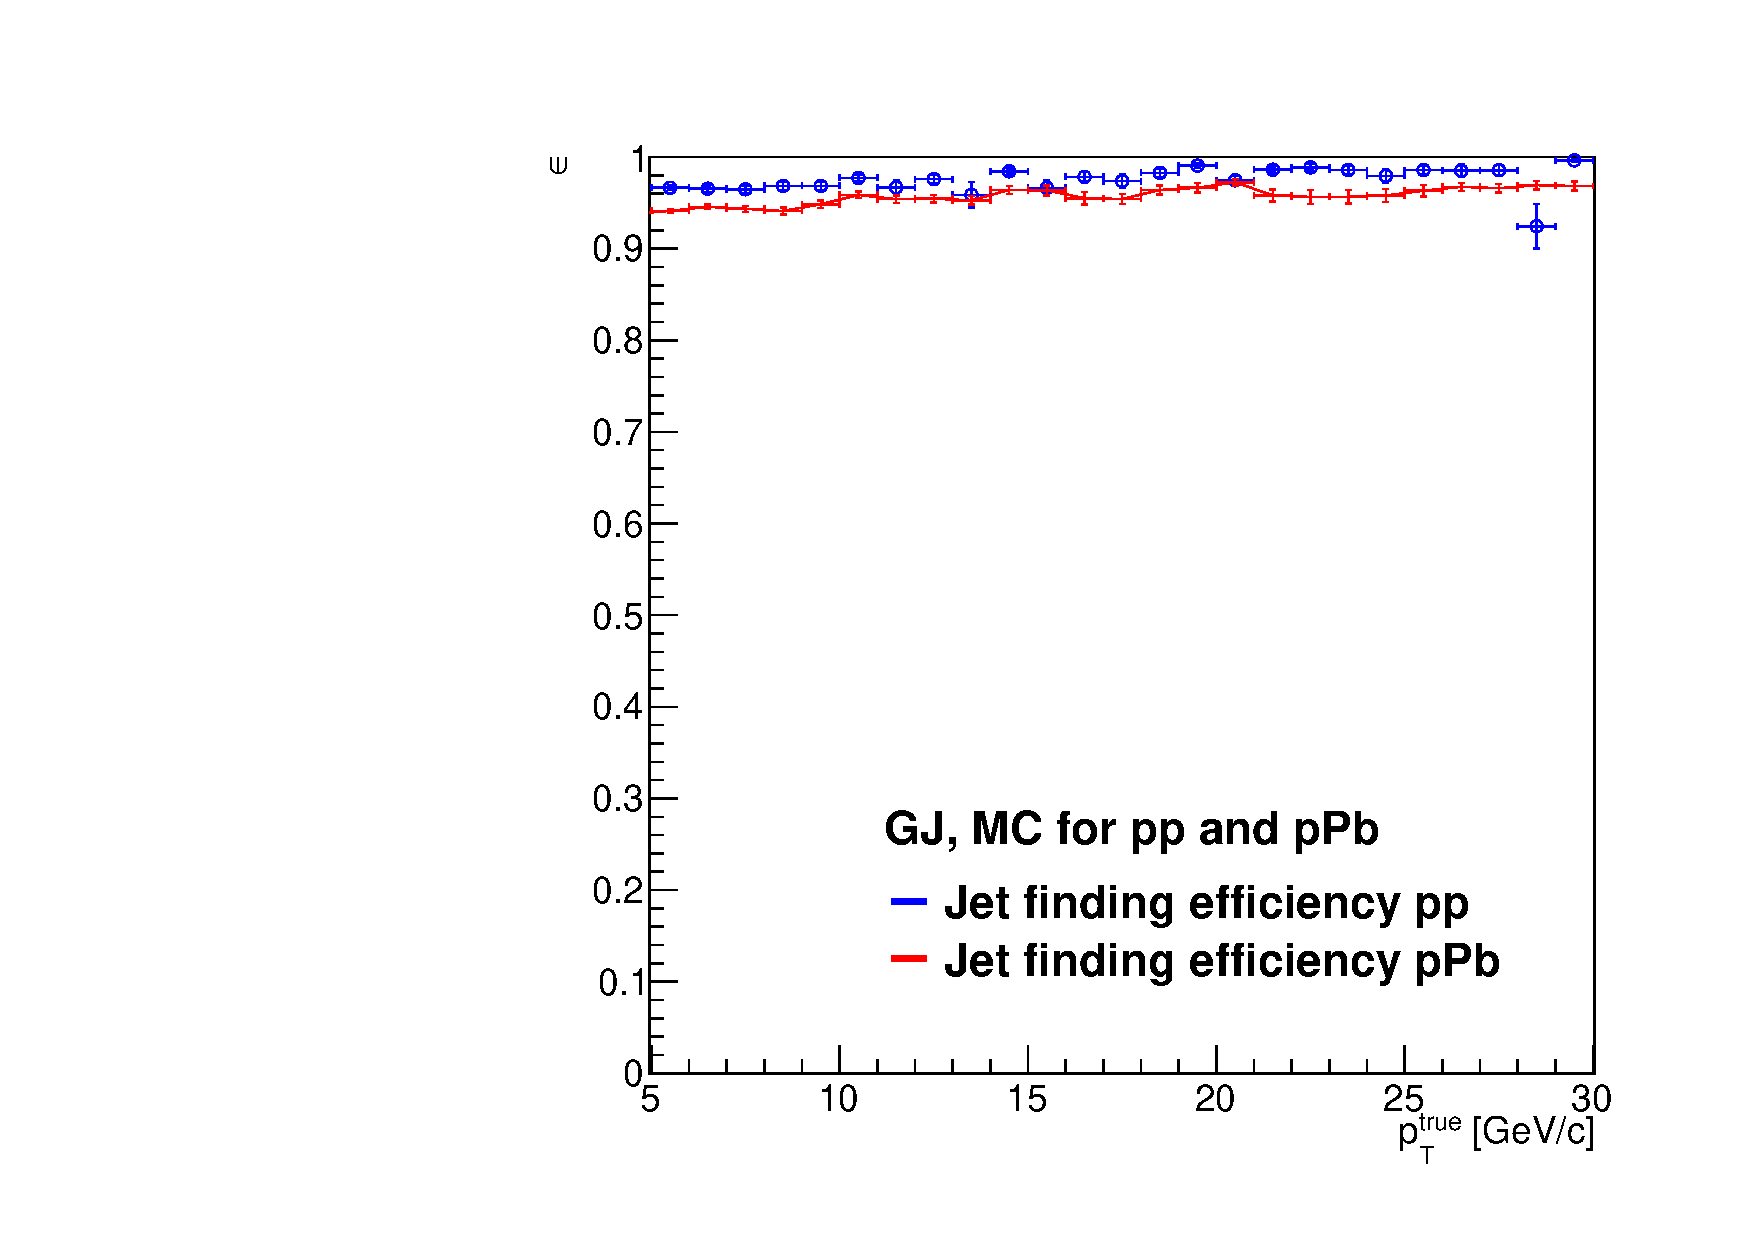
\includegraphics[width=.495\textwidth]{JetResponse/jet_findEff_its.pdf}
\caption{The Jet finding efficiency in both pp and p-Pb as a function of $\pt^{\mathrm{true}}$ for 5 \GeVc $<\pt^{\mathrm{true}}<$ 30 \GeVc, using LHC17g6a1 and LHC18b10a for p-Pb and pp respectively. The efficiency is greater than 90\% for both pp and p-Pb jets.}
\label{fig:jetfindingEff}
\end{figure}












